\section{Introduction}
The aim of this experiment is to analyze particle physics processes over real and simulated events from the ATLAS experiment. The study began by learning how particles leave their tracks in the detector, sample data for electron, muon, photon, tau and jet events were examined. Then, the energy losses of muons were analyzed, and electron-positron pairs from Z boson decays were used for calibration purposes. Finally, event-based interpretations were made on the data set called the “mystery dataset” and possible Standard Model processes were tried to be determined. Then $Z$ boson mass calibraiton tried to achieved to use for measuring the $W$ boson mass.

\section{Preparation}

\section{Overview and Event Display}
\label{sec:eventdisplay}

Before starting to main task of this experiment, initially event display of the particle reactions were investigated. For this purpose, five different data sets searched and tried to be familiarised to how particles reaction visualized on the display. These learning data sets are not real data sets and can be listed as electrons, muons, photons, $\tau$ leptons and jets \cite{atlaslabmanual}. \\

Event display mainly shows the crosssection of the detectors and tracking systems as can be seen from fig.\ref{fig:eventdisplay_Learning}. From center of the detector to outside, components of the ATLAS detector consists of Pixel Detector, Semi-Conductor Tracker (SCT), Transition Radiation Detector (TRT) in the inner part which is inside area of the green circle on event display.
Following these components, there are electromagnetic calorimeter (ECAL) and hadronic calorimeter (HCAL) which are shown green and red areas on the event display consecutively. Finally, the outermost layer is the muon detector system, or muon spectrometer \cite{atlaslabmanual}.

\subsection{Electrons}
\label{subsec:Electrons_disp}
On the fig.\ref{fig:LearningData_electron}, the reaction of an electron with the ECAL of the ATLAS detector can be seen. When a single electron is produced in the ATLAS detector, it first leaves a clear track in the inner detector (light blue line). This track is formed due to the charge of the electron, and the direction and magnitude of its momentum are measured from this track. Then, when the electron hits the ECAL, it produces an intense electromagnetic shower (yelow area in ECAL). This shower is measured by using liquid Argon (LAr) and the energy of the electron is determined. Typically, electrons leave very little energy in the HCAL, therefore, this is a criterion for distinguishing between electrons and hadrons.

\begin{figure}[h]
	\begin{subfigure}{0.45\textwidth}
		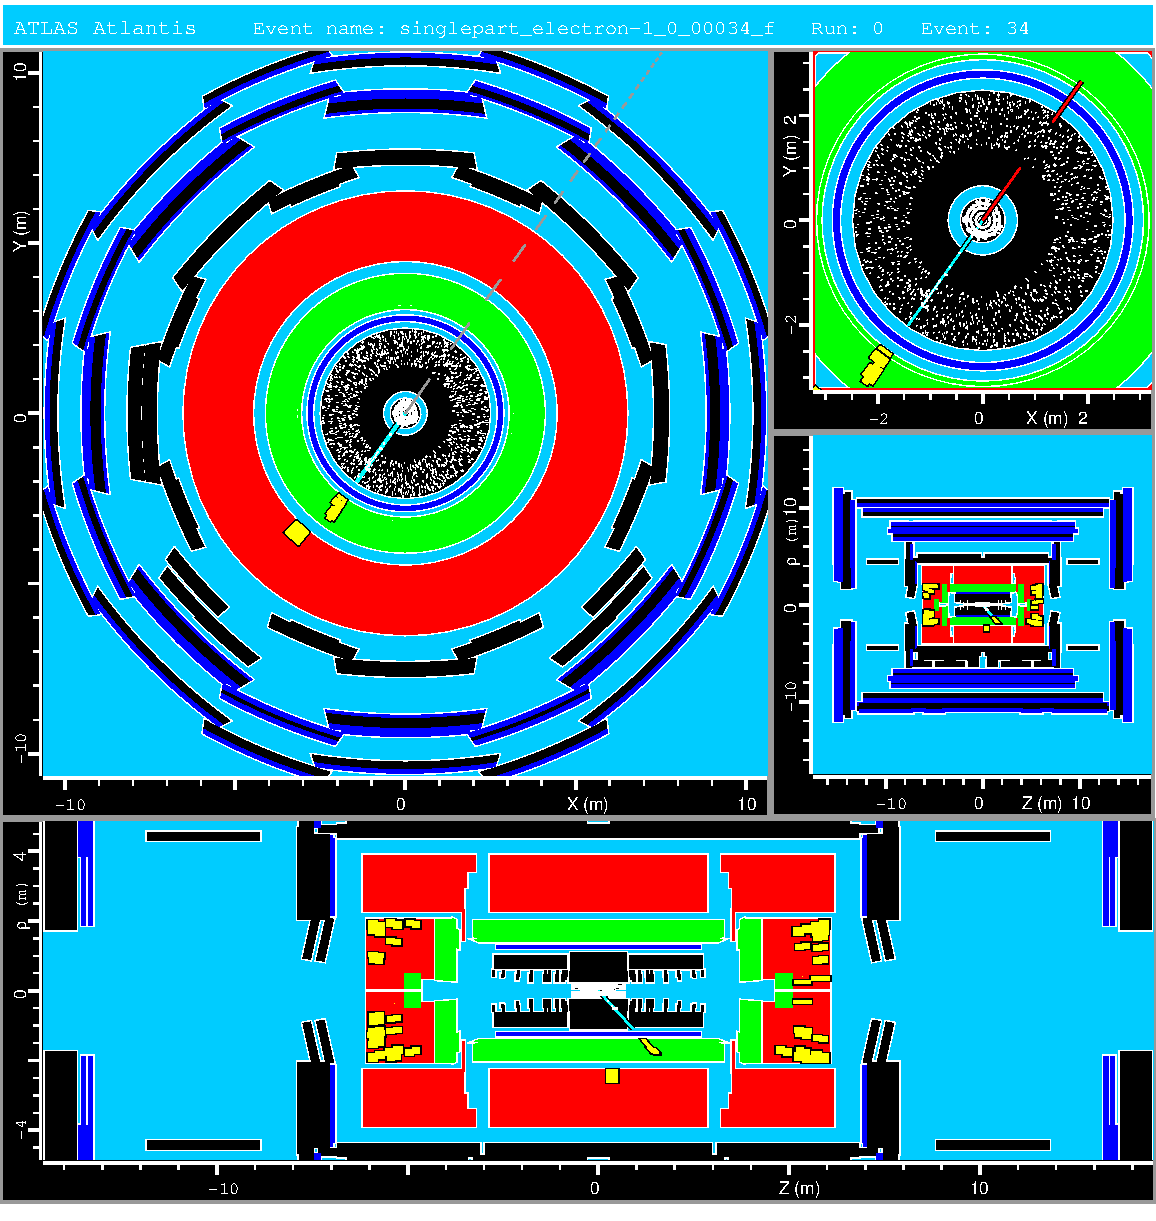
\includegraphics[width=\textwidth]{../figures/LearningData_electron.pdf}
		\caption{single-electron}
    		\label{fig:LearningData_electron}
	\end{subfigure}
	\hfill
	\begin{subfigure}{0.45\textwidth}
	 	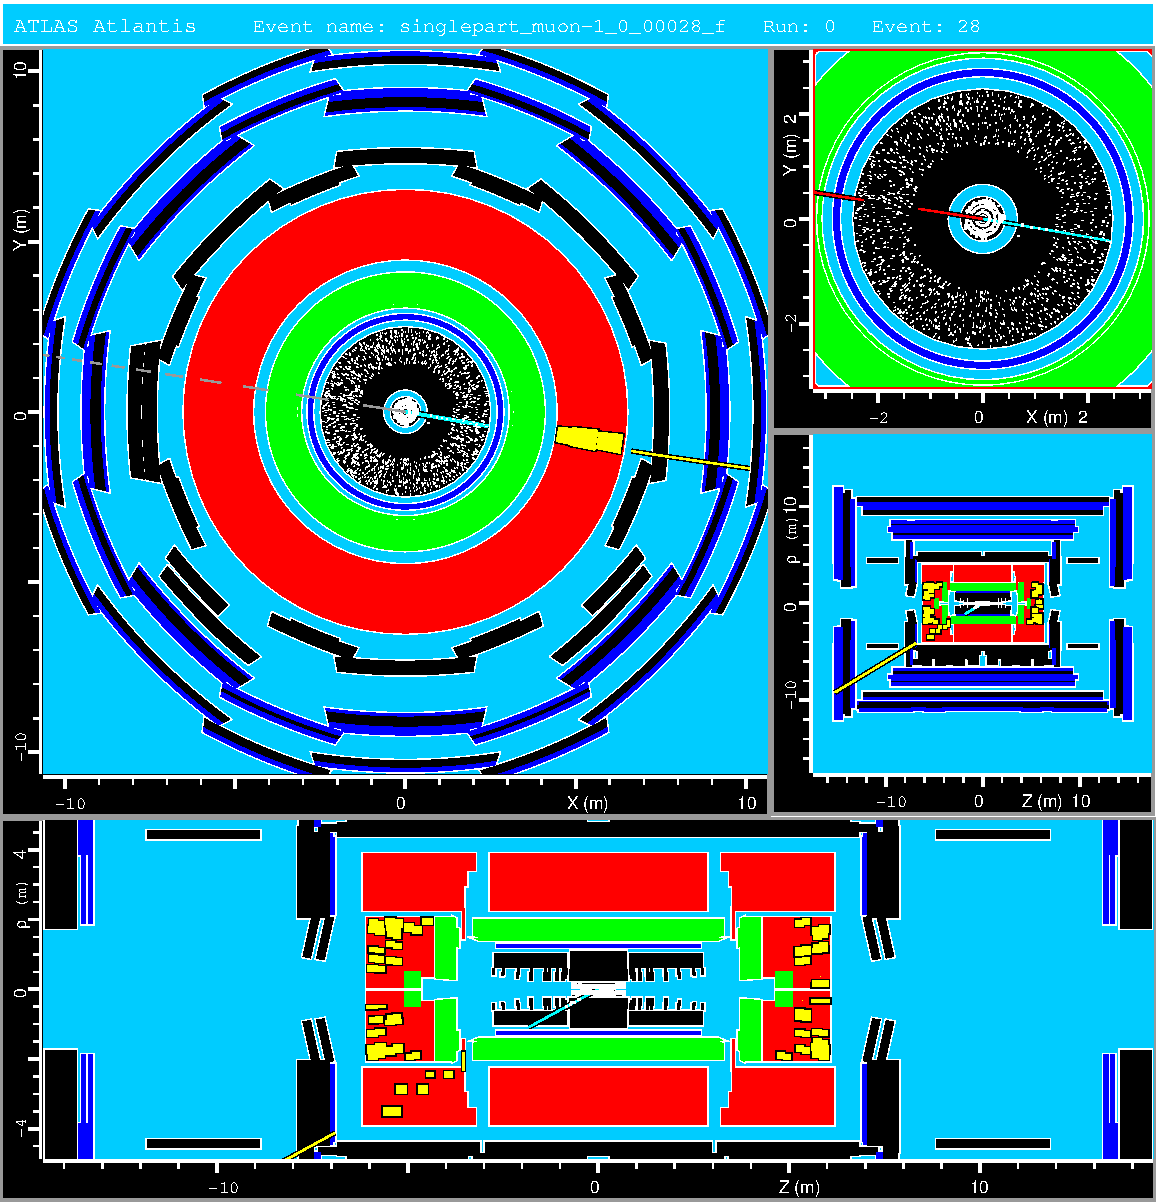
\includegraphics[width=\textwidth]{../figures/LearningData_muon.pdf}
		\caption{single-muon}
		\label{fig:LearningData_muon}
	\end{subfigure} 
	\hfill
	\begin{subfigure}{0.45\textwidth}
    		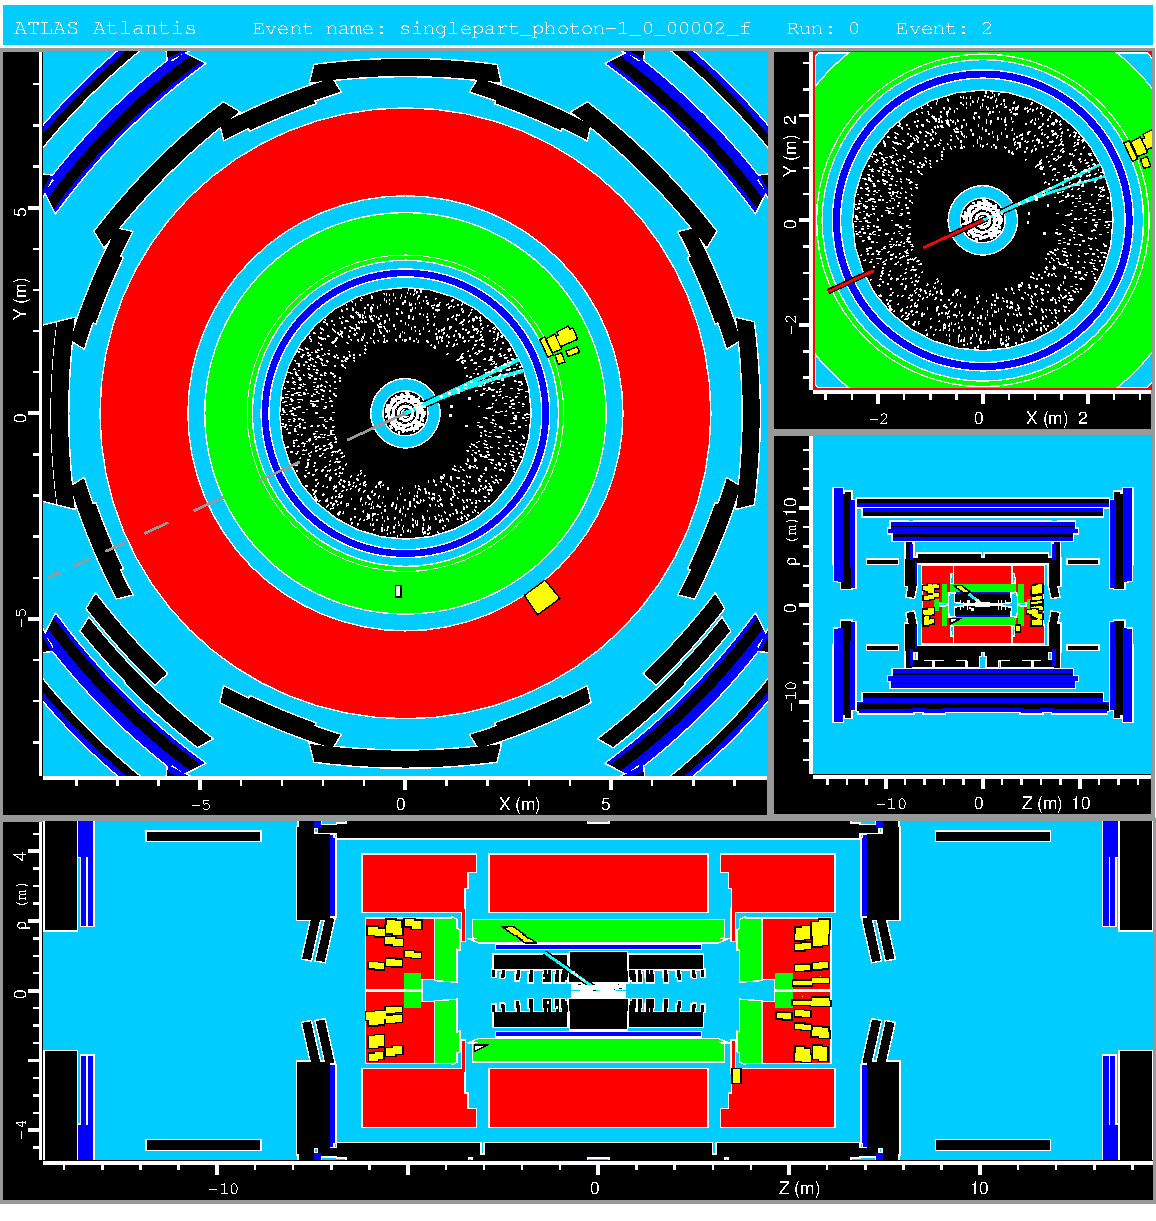
\includegraphics[width=\textwidth]{../figures/LearningData_photon.pdf}
		\caption{single-photon}
		\label{fig:LearningData_photon}
	\end{subfigure} 
	\hfill
	\begin{subfigure}{0.45\textwidth}
		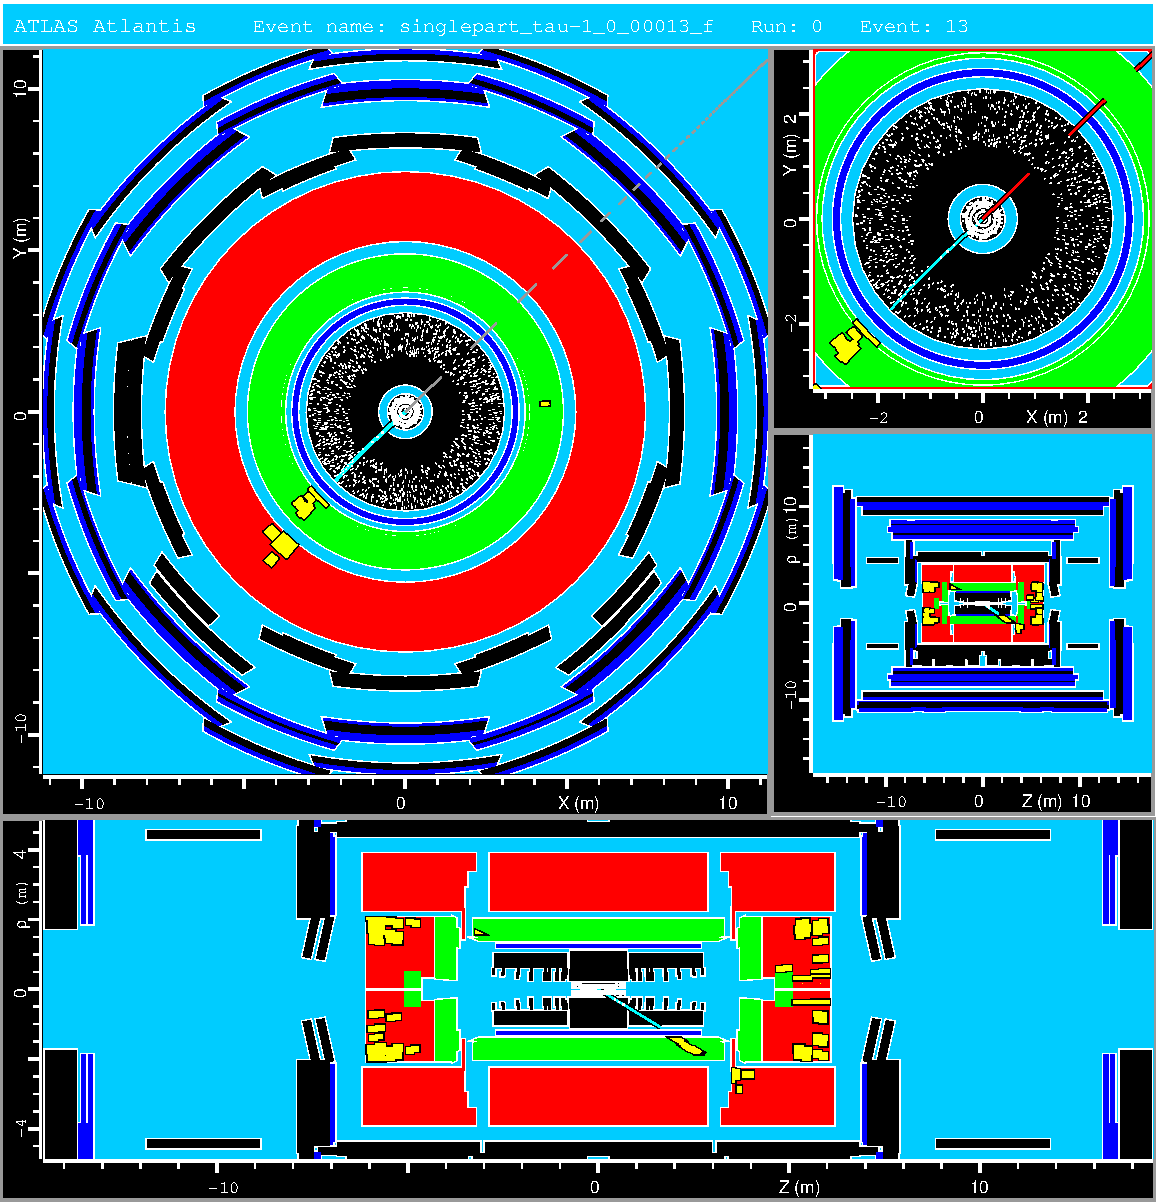
\includegraphics[width=\textwidth]{../figures/LearningData_tau.pdf}
		\caption{single $\tau$ lepton}
		\label{fig:LearningData_tau}
	\end{subfigure} 
	\hfill
	\begin{subfigure}{0.45\textwidth}
		\centering
		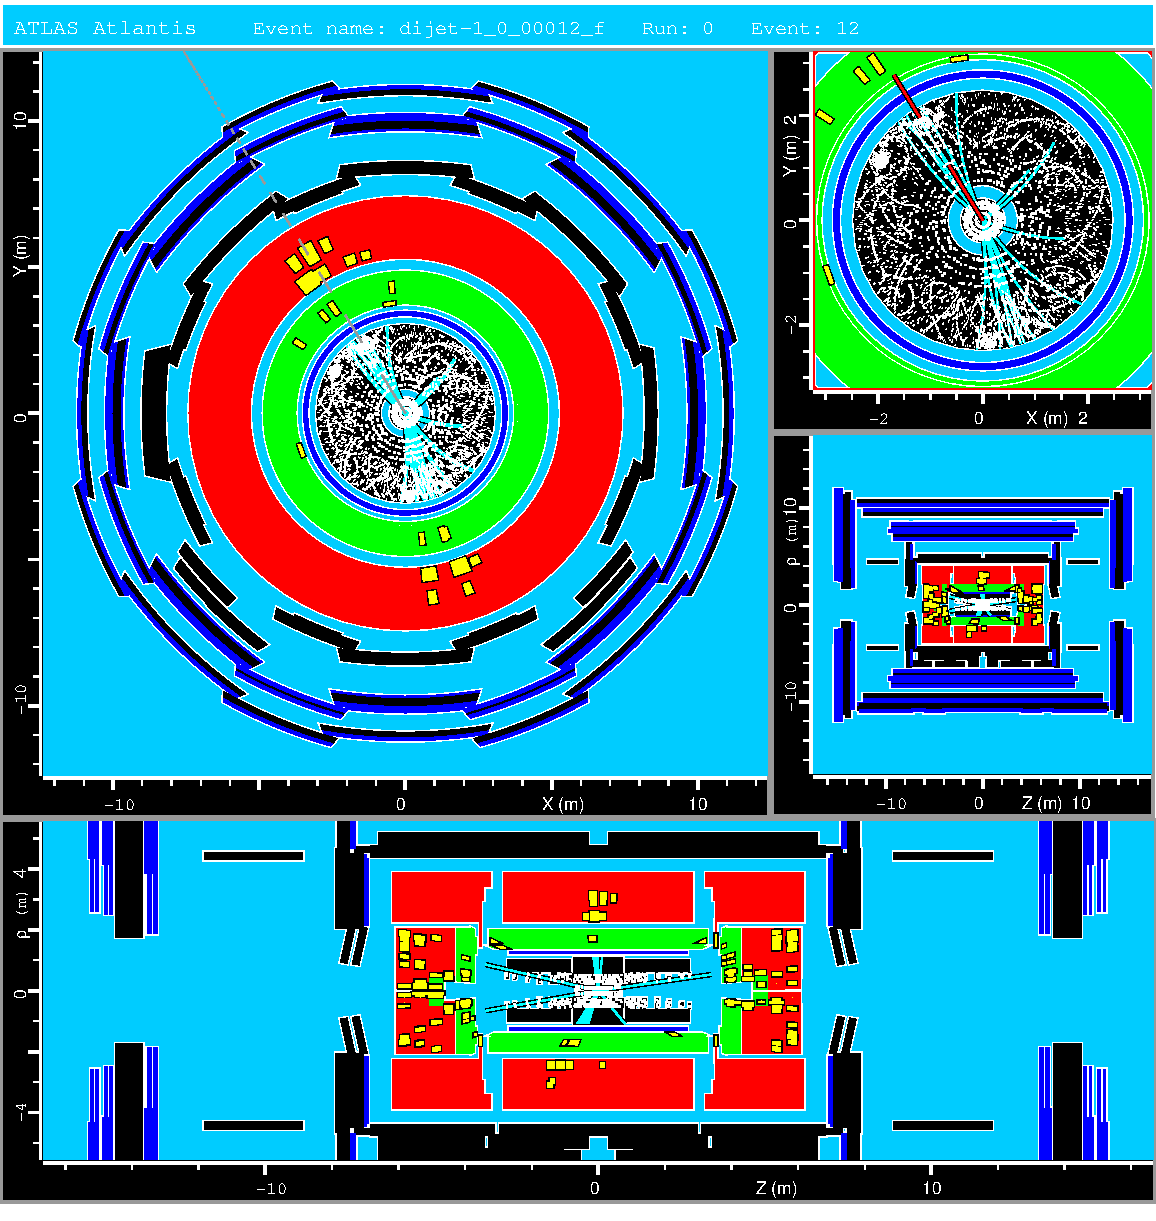
\includegraphics[width=\textwidth]{../figures/LearningData_dijet.pdf}
		\caption{dijet}
		\label{fig:LearningData_dijet}
	\end{subfigure}
	\caption{Event display images of \texttt{ATLANTIS} program for five different learning data sets.}
	\label{fig:eventdisplay_Learning}
\end{figure}
\FloatBarrier

\subsection{Muons}
\label{subsec:Muons_disp}
When a muon is produced in the ATLAS detector, it first leaves a regular track as a charge-carrying particle in the inner detector system (light blue line) as seen in the fig.\ref{fig:LearningData_muon}. However, unlike electrons, muons leave very little energy in ECAL and HCAL, because they interact weakly in these environments and pass through without losing most of their energy. Therefore, minimal energy accumulation is seen in the calorimeters in a muon event. After the muons pass through these layers, they are detected by the muon spectrometer, which is located in the outermost part of the detector and is specifically designed to detect muons. Here, their tracks (yellow line on fig.\ref{fig:LearningData_muon}) are measured again under large magnetic fields and their charges and momentums are determined. In this way, the match of the tracks seen in both the inner detector and the muon system confirms the presence of a muon.


\subsection{Photons}
\label{subsec:Photons_disp}
When a photon enters the ATLAS detector, it does not leave a trace in the inner detector system because it does not carry an electric charge. However, when it reaches the ECAL, it creates electron-positron pairs there, initiating an electromagnetic shower (EM shower). This shower expands within the ECAL, producing secondary particles, and the detector measures the energy left by these particles. If the photon has a high energy, the shower can be noticeable. The photon has little effect on the hadronic calorimeter (HCAL), because it does not interact with the hadrons. If a photon is to be confused with another particle that behaves like an electron, a trace is investigated in the inner detector. Therefore, if an EM shower is observed but no trace is found in the inner detector, this is a photon signature. On the other hand, sometimes photons interact with the inner detector and creates electron-positron pairs, and these particles also creates an EM shower on the ECAL \cite{hanagaki2023pid}. This seems the case in the fig.\ref{fig:LearningData_photon}. Because there are traces in the inner detectors.


\subsection{\texorpdfstring{$\tau$}{tau}-leptons}
\label{subsec:tauleptons_disp}
$\tau$-leptons are the heaviest leptons in the Standard Model and have very short lifetimes (about $10^{-13}$ seconds). Therefore, they are not directly observed in the ATLAS detector because they decay before reaching the active regions of the detector. $\tau$-leptons decay to produce either an electron or a muon and a neutrino which is called as leptonic decay, or several hadrons and a neutrino called as hadronic decay. In leptonic decays, the resulting electron or muon is directly observed in the detector, and the neutrino is not visible in the detector, contributing to missing transverse energy, $\slashed{E}_T$. In hadronic decays, a narrow hadronic jet is observed. This jet is usually narrower than ordinary QCD jets and can be distinguished by this feature. Therefore, $\tau$-leptons are indirectly detected in ATLAS by combinations of decay products and $\slashed{E}_T$. In the fig.\ref{fig:LearningData_tau}, a neutrino trace (dashed line) is observed, and in the reverse direction there are energy accumulation on ECAL and HCAL. It is hard to understand without knowing energy accumulation in ECAL and HCAL, if this is a hadronic or leptonic decay of $\tau$.


\subsection{Dijets}
\label{subsec:jets_disp}
Dijet events consist of two hadronic structures (jets) that are produced by the scattering of two quarks or gluons in proton-proton collisions, and forming a jet. In the ATLAS detector, these jets are observed as large energy deposits in the HCAL, because the quarks and gluons produce large numbers of particles as they transform into hadrons, or called as hadronization. The jets may also left some energy in the ECAL, but most of the energy is absorbed in the HCAL. $\slashed{E}_T$ in such events is usually low because all the energy can be measured by the detector. Dijets usually shows themselves as pairs of symmetric high-energy jets as can be seen from the fig.\ref{fig:LearningData_dijet}.


\section{Preparatory Questions}
\label{sec:prepquest}
In the following questions were asked for a preparation to main part of the lab, and answered as follows. 


\subsection{Question A: Decay of a $Z^0$ boson}
\label{sec:QuestionA}
\textbf{Which value does the momentum of an electron have in the decay of a $Z^0$ boson  $Z^0\rightarrow e^+e^-$, if the $Z^0$ is at rest?} \cite{atlaslabmanual}\\
In the process of decaying of $Z^0$, a pair of an $e^-$ and a $e^+$ is obtained, and during this process 
4-vector momentum must be conserved as in eqn. \ref{eqn:4vecmom}.
\begin{equation}
	\label{eqn:4vecmom}
	\mathbf{P_{Z^0}} = \mathbf{P_{e^+}} + \mathbf{P_{e^-}}
\end{equation}
more explicit way eqn. \ref{eqn:4vecmom} can be written as,
\begin{equation}
	\label{eqn:4vecmom_exp}
	\begin{pmatrix} M_{Z^0} \\ 0 \\ 0 \\ 0  \end{pmatrix}=
	\begin{pmatrix} E_{e^+} \\ p_{e^+_x}\\p_{e^+_y}\\p_{e^+_z} \end{pmatrix} +
	\begin{pmatrix} E_{e^-} \\ p_{e^-_x}\\p_{e^-_y}\\p_{e^-_z} \end{pmatrix} 
\end{equation}


Initially, $Z^0$ boson is at rest, hence, $E_{Z^0}=M_{Z^0}$.
On the other hand, obtained $e^-$ and $e^+$ have same amount of momentum but in opposite directions due to the momentum conversation $\left(\mathbf{p_{e^+}}=-\mathbf{p_{e^-}}\right)$, and have same amount of energy, $\left(E_{e^+}=E_{e^-}=E_{e}\right)$.
Therefore, relation in the below eqn. \ref{eqn:enmom} can be obtained from eqn. \ref{eqn:4vecmom_exp}.
 \begin{equation}
	 \label{eqn:enmom}
	 E_{e} = \frac{M_{Z^0}}{2}
\end{equation}
using energy momentum relation, $E^2 = p^2 + M^2$, the electron momentum after decaying process can be obtained as,
\begin{equation}
	\label{eqn:ElMom}
	p_e = \sqrt{E_e^2 + M_e^2}
\end{equation}

implementing eqn. \ref{eqn:enmom} to  eqn. \ref{eqn:ElMom}, final result is gained as

\begin{equation}
       \label{eqn:finElMom}
	p_e = \sqrt{\left(\frac{M_{Z^0}}{2}\right)^2 + M_e^2}
\end{equation}

Mass of the $Z^0$ boson has a value of $M_{Z^0} = 91.1876 \pm 0.0021 \text{GeV/$c^2$}$\cite{pdg2018}, and mass of the electron has a value of $M_e = 0.510 998 950 69(16) \text{MeV/$c^2$}$\cite{nistmec2}.

Hence, $p_e= 45.5966 \pm 0.0011 \text{Gev/c}$. In this calculation, $M_e$ negligibly small when compared to $M_{Z^0}$ so the electron and pozitron almost has a momentum of the half of the $Z^0$ boson mass in decaying process.  



\subsection{Question B: Scattering reaction $e^+e^- -> τ^+τ^-$}
\label{sec:QuestionB}
\textbf{How large is the momentum of tau leptons in the reaction $e^+e^- \rightarrow \tau^+\tau^-$ , if the reaction takes place in the center-of-mass system (center-of-mass energy = 5 GeV)?} \cite{atlaslabmanual}\\

In the scattering process of $e^+e^- \rightarrow\tau^+\tau^-$ in the fig.\ref{fig:elecpositscatter}, 4-vector momentum again must conserved.
\begin{figure}[h]
    \centering
    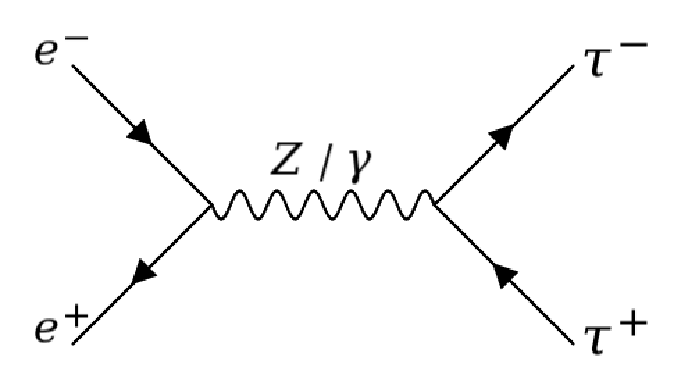
\includegraphics[width=0.5\textwidth]{../figures/elecpositscatter.pdf}
	\caption{Feynman diagram of $e^+e^- \rightarrow\tau^+\tau^-$}
    \label{fig:elecpositscatter}
\end{figure}
\FloatBarrier

\begin{equation}
	\label{eqn:4momConsB}
	\mathbf{P_{CM}} = \mathbf{P_{\tau^+}} + \mathbf{P_{\tau^-}}
\end{equation}

$\mathbf{P_{CM}}$ is the 4-vector center of mass momentum, and can be defined as in eqn. \ref{eqn:4vecmomB},

\begin{equation}
	\label{eqn:4vecmomB}
	\mathbf{P_{CM}} = \begin{pmatrix} E_{CM} \\ 0 \\ 0 \\ 0  \end{pmatrix} \quad
	\mathbf{P_{\tau^+}} = \begin{pmatrix} E_{\tau} \\ p_{\tau^+_x}\\p_{\tau^+_y}\\p_{\tau^+_z} \end{pmatrix} \quad
	\mathbf{P_{\tau^-}} = \begin{pmatrix} E_{\tau} \\ p_{\tau^-_x}\\p_{\tau^-_y}\\p_{\tau^-_z}  \end{pmatrix}
\end{equation}

Therefore, using momentum conservation, $\left(\mathbf{P_{CM}}\right)^2 = \left(\mathbf{P_{\tau^+}} + \mathbf{P_{\tau^-}}\right)^2$, eqn. \ref{eqn:questionB22} is obtained.

\begin{equation}
	\label{eqn:PcmB}
	E_{CM}^2 = \left( 2E_{\tau} \right) ^2
\end{equation}

\begin{equation}
	\label{eqn:questionB21}
	E_{CM}^2 = 4m_{\tau}^2 + 4p_{\tau}^2
\end{equation}

\begin{equation}
	\label{eqn:questionB22}
	p_{\tau} = \frac{1}{2}\sqrt{E_{CM}^2-4m_{\tau}^2}
\end{equation}

$m_{\tau}=1777.09\pm0.14$ MeV/$c^2$ \cite{belle2_taumass2023}, and $E_{CM} = 5$ GeV/$c^2$ \cite{atlaslabmanual}. Hence, momentum of the $\tau$-leptons are

\begin{equation}
	\label{eqn:taumomB}
	p_{\tau} = 1.75839 \pm 0.00056 \text{GeV/$c^2$}
\end{equation}

\subsection{Question C: Tree variable \texttt{ptw}}
\label{sec:QuestionC}
\textbf{As before, the analysis is based on ROOT trees. One of the tree variables is ptw -
the estimated transverse momentum of the W boson candidate. This variable can
be constructed from the other tree variables. Please think about how this could be
done.} \cite{atlaslabmanual} \\

The transverse momentum of the $W$ boson, is can be described with the electron momentum and the neutrino momentum 
\begin{align*}
    \vec{p}_{T,W} = \vec{p}_{T,e} + \vec{p}_{T,\nu}
\end{align*}
The transverse momentum of electron and neutrino is made up of a part in x and a part in y direction. So the value of the  $\left|\vec{p}_{T,W}\right|$ can be calculated
using 
\begin{align*}
    |\vec{p}_{T,W}| = \sqrt{(p_{T,e,x} + p_{T,\nu,x})^2 + (p_{T,e,y} + p_{T,\nu,y})^2}.
\end{align*}
Since the neutrino momentum can't be measured directly in the detector, this missing transverse momentum is used. 
Inserting the corresponding ROOT variables in the expression, $\left|\vec{p}_{T,W}\right|$ can be constructed with 
\begin{align*}
    \texttt{ptw} = \sqrt{(\texttt{el\_px} + \texttt{ptmisx})^2 + (\texttt{el\_py} + \texttt{ptmisy})^2}.
\end{align*}

\subsection{Question D: Gaussian error propagation for correlated parameters}
\label{sec:QuestionC}
\textbf{Please look up the correct form of the Gauss
error propagation law in the presence of correlations. You will need that for the final error
on the W mass.} \cite{atlaslabmanual} \\
If a function f(a,b) has uncertainties $\sigma_a$ and $\sigma_b$, which are correlated, the gaussian error propagation for correlated uncertainties is given by
\begin{equation*}
\sigma_f^2 = \left( \frac{\partial f}{\partial a} \cdot \sigma_a \right)^2 + \left( \frac{\partial f}{\partial b} \cdot \sigma_b \right)^2 + 2 \cdot \frac{\partial f}{\partial a} \cdot \frac{\partial f}{\partial b} \cdot \sigma_{ab}
\end{equation*}

\section{Assignments on Particle Reactions}

\section{Measured $µ$ Momentums and Energy Loss}
\label{sec:muonmom}

In order to investigate the energy loss of muons, energy measurements of $20$ consecutive events in the
\texttt{muon learning} dataset were compared. In this analysis, the differences between the momentum
measured in the inner detector and the momentum measured in the muon spectrometer were
evaluated. Both detectors determine the momentum by following the trajectory of the muons with the
help pf a magnetic field. Transverse, $p_T$, and total momentum, $p$, values are derived from the
curvature of the curved track of the charged particle. These values were obtained from the each event
using \texttt{ATLANTIS} program.

The dataset was selected to include as many consecutive events as possible. However, since the detectors could not detect the energy measurement in some events, these events were excluded from the analysis. In particular, missing measurements were detected in events $3$, $10$, $14$ and $21$, and this data set can be seen in the tab.\ref{tab:innerdetector} and tab.\ref{tab:muondetector}. The measured negative momenta are generally associated with $\mu^-$, and the positive momenta with $\mu^+$. Thus, the momenta observed in each event also contributes to the indirect determination of the particle’s charge.

In the fig.\ref{fig:EnergyLoss}, the events belonging to muons are analyzed. The horizontal axis shows the event number, while the vertical axis shows the difference between the momentum measured in the inner detector and the momentum measured in the outer muon detector for each event, or the energy loss. This difference is usually positive due to the weak interaction of muons with the detector materials, since muons mostly lose their energy through ionization. The red horizontal line in the graph represents the average energy loss and equal to $3\pm6$GeV/$c^2$. The light magenta band shows the standard deviation range of $\pm1\sigma$, and determined by the Gaussian error propagation. Remarkably, all measurements except $3$ data points intercept with this band. This shows that the measurements largely follow the expected statistical distribution.

\begin{figure}[h]
    \centering
    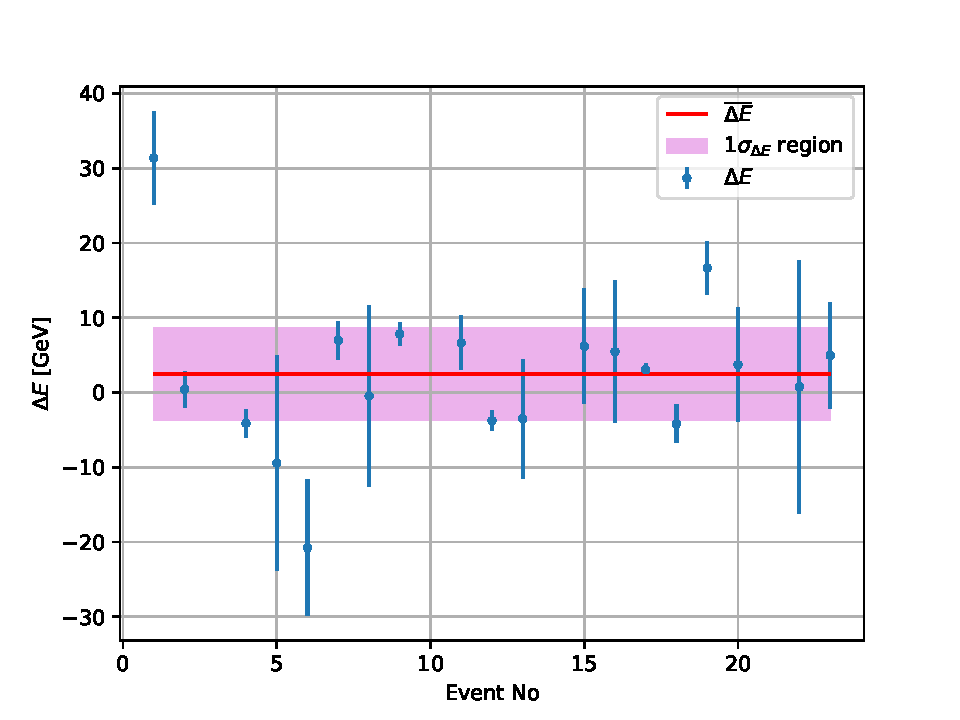
\includegraphics[width=\textwidth]{../figures/EnergyLoss.pdf}
	\caption{Energy loss of muons in the ATLAS detector corresponding to each event number. Red lines shows the average energy loss, and most of the measurements stand inside the $\pm1\sigma$ error range.}
    \label{fig:EnergyLoss}
\end{figure}
\FloatBarrier



However, in some events the energy difference is negative. This situation can occur for various reasons. First, it can be due to systematic errors in the momentum measurement or differences in detector resolution. In particular, although the magnetic field in the inner detector provides a more sensitive measurement, deviations can occur. A second possibility is that the momentum measurement in the outer detector appears higher than it actually is due to magnetic field or timing differences. Finally, particle tracks or residual signals within the event may also disurb the measurement in the outer detector.

Even though errors for $p_T$ were provided by the \texttt{ATLANTIS} program, errors for total momenta, $p$ was not provided. It is assummed that error propagation of the transverse momentum, $p_T$, is the same with error propagation of total momentum. Therefore, errors for total momentum calculated as in eqn.\ref{errorprop}.

\begin{equation}
	\label{errorprop}
	\frac{\sigma_{p_T}}{p_T}=\frac{\sigma_p}{p}
\end{equation}



\section{Mystery Data Set}
\label{sec:mystery}
The dataset named \texttt{Mystery-xxx.dat} was prepared to examine possible physical processes in the Standard Model. A pre-selection was applied to this dataset in advance, and it is known that at least two leptons ($e$ and $\mu$) are present in each event. The aim of this study is to determine which Standard Model process could cause these events by using the distinctive features of the leptons, jets, or $\slashed{E}_T$ \cite{atlaslabmanual}. For this purpose, events numbered $6$, $11$, $20$, and $45$ were selected and examined.

\subsubsection{Event 6:}

\begin{figure}[h]
    \centering
	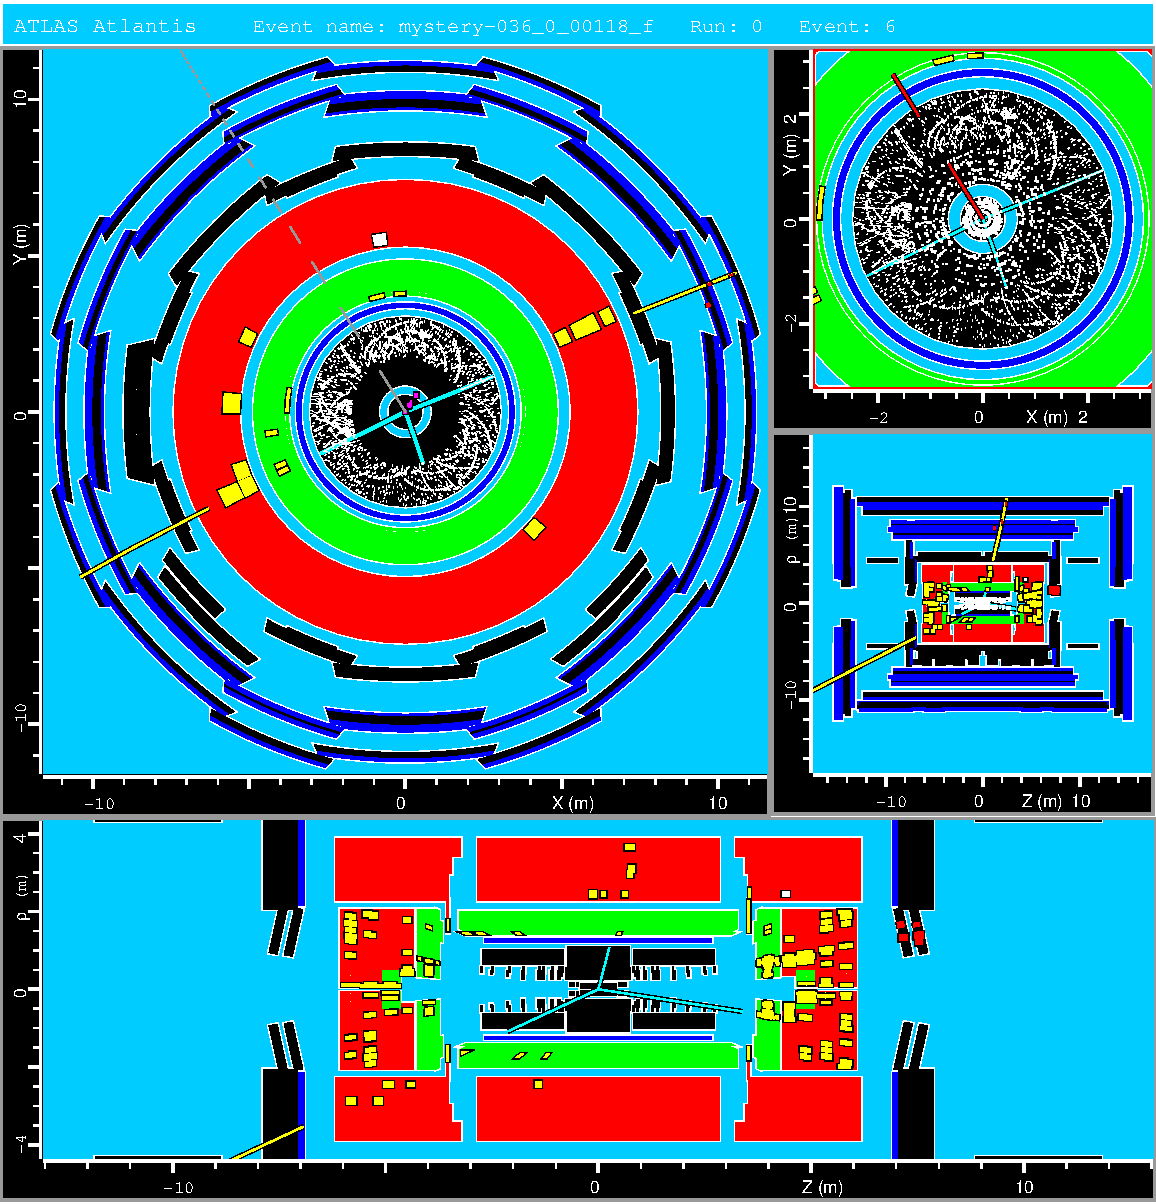
\includegraphics[width=0.5\textwidth]{../figures/mystery-event6.pdf}
	\caption{Mystery data set \texttt{Event 6}}
    \label{fig:event6}
\end{figure}
\FloatBarrier

Two muons are observed in this event. Since the $\slashed{E}_T$ was measured as $2.082$ GeV which is quite small, the probability of a neutrino presence in the event is low. Also, the muons are moving in opposite directions. This suggests that the event may be a Drell-Yan process for pair production as can be seen from fig.\ref{fig:DrellYan001}. In this process, a virtual photon, $\gamma^*$ or $Z$ boson is created by the scattering of one quark anti-quark pair, then this boson (or photon) decays into a lepton pair (here two muons). If the event was a $W$ boson, a neutrino would be expected among the decay products. However, the low $\slashed{E}_T$ observed indicates that there is no such neutrino contribution.

\begin{figure}[h]
    \centering
	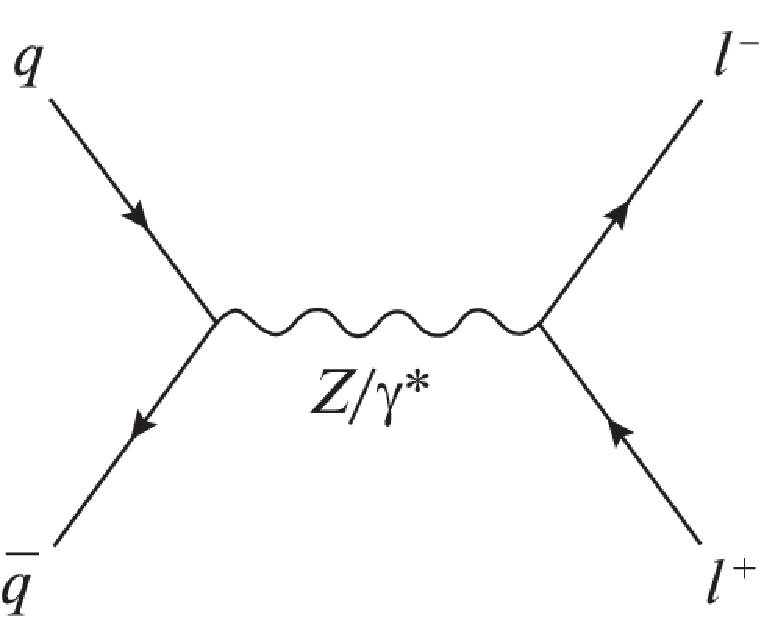
\includegraphics[width=0.5\textwidth]{../figures/DrellYan001.pdf}
	\caption{Drell-Yan Processes of a $Z$-boson or photon decaying to a lepton pair. Figure was taken from \cite{shalaev2021drellyan}}
    \label{fig:DrellYan001}
\end{figure}
\FloatBarrier
Also, it must be noted that these two particles deposited low energies on the calorimeters. For left muon deposited energy smaller than $5$ GeV, and for right muon smaller than $3$ GeV. On the other hand, $p_T$ was measured for right muon as $-21.83 \pm 1.413$ GeV, and for left muon as $45.06 \pm 3.807$ GeV. These opposite signed energy values shows that these two particles have opposite charges, and smaller deposited energies on the calorimeters  also shows that these two particles are actually muons.


\subsubsection{Event 11:}

\begin{figure}[h]
    \centering
    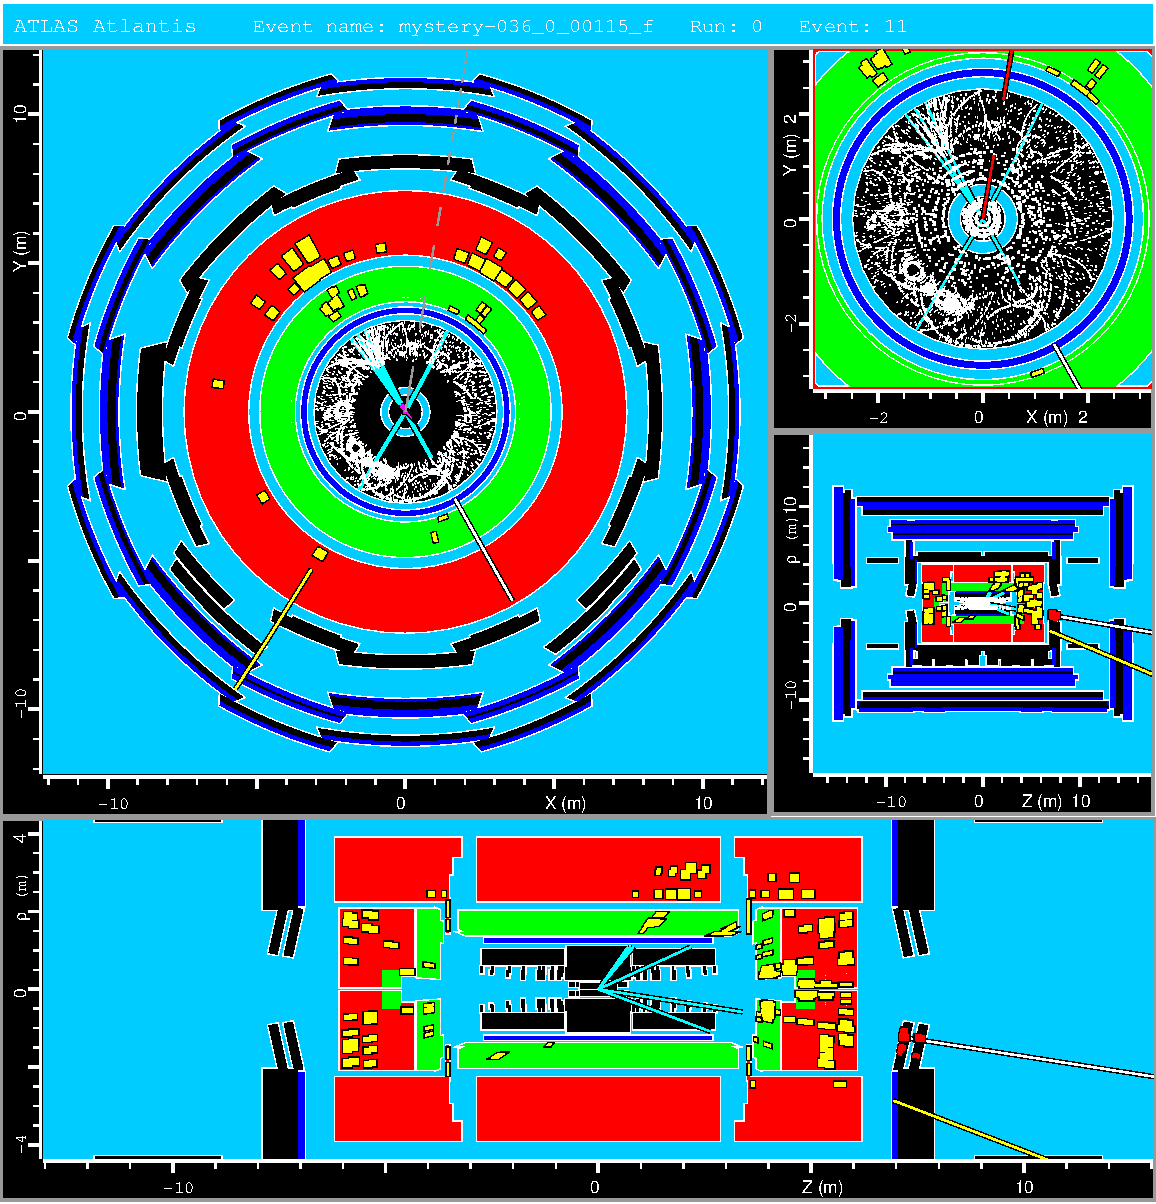
\includegraphics[width=0.5\textwidth]{../figures/mystery-event11.pdf}
	\caption{Mystery data set \texttt{Event 11}}
    \label{fig:event11}
\end{figure}
\FloatBarrier
On the upper side of the event display, there are two jets formations are seen. On the bottom side again two muons were observed due to same reasons before: small energy deposition on calorimeters and high $p_T$ values can be seen from below tab.\ref{tab:event11}

\begin{table}[h]
		\centering
        \begin{tabular}{cc}
            \toprule
             product & Energy information [GeV]  \\
            \midrule
            bottom left $\mu$ & $p_T = -41.55 \pm 5.129$  \\
  			\midrule
  			bottom right $\mu$ & $p_T = 121.40 \pm 3.258$   \\
  			\midrule
  			top left jet & $ 21.1$(ECAL)  $ 37.0$(HCAL) \\
  			\midrule
  			top right jet & $ 8.9$(ECAL)  $ 19.5$(HCAL) \\
  			\midrule
  			possible $\nu$ & $\slashed{E}_T = 23.773$ \\
			\bottomrule
        \end{tabular}
        \caption{Energy information of particles in \texttt{Event 11}, values were obtained via \texttt{ATLANTIS} program}
        \label{tab:event11}
    \end{table}
\FloatBarrier

This process cannot be basically leptonic pair production from $Z$ boson or a photon. Because there are two jet formations and a possible neutrino were observed besides two muons. Possible processes can be considered as quark and antiquark scattering or gluon-gluon fusion can be described as in the eqn.\ref{eqn:qqscatter}, and eqn.\ref{eqn:ggfusion}. Feynman diagrams of these processes can be seen from the fig.\ref{fig:possibleProc11}.

\begin{equation}
	q\bar{q} \rightarrow g \rightarrow t\bar{t} \rightarrow bW\bar{b}W \rightarrow b\mu\nu_\mu\mu\nu_\mu\bar{b}
	\label{eqn:qqscatter}
\end{equation}

\begin{equation}
	gg \rightarrow b\bar{b}b\bar{b} \rightarrow bZWc \rightarrow b\mu^+\mu^-e\nu_ec
	\label{eqn:ggfusion}
\end{equation}

In the eqn.\ref{eqn:qqscatter}, two $b$ quarks can be the responsible from the jet formations and there is chance that one of the neutrino could not be detected.

Same in eqn.\ref{eqn:ggfusion}, one $b$ and one $c$ quarks can be responsible from the jet formations, and the $e$ could not be detected.

\begin{figure}[h]
	\begin{subfigure}{0.45\textwidth}
		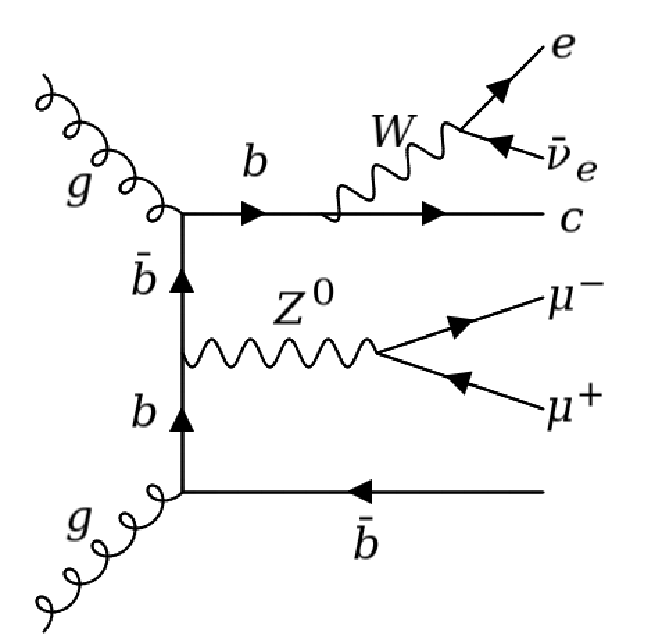
\includegraphics[width=\textwidth]{../figures/ggFusion.pdf}
		\caption{$gg$ fusion to $b$ quarks and $Z$ boson and their decaying processes.}
    		\label{fig:ggfusion}
	\end{subfigure}
	\hfill
	\begin{subfigure}{0.45\textwidth}
	 	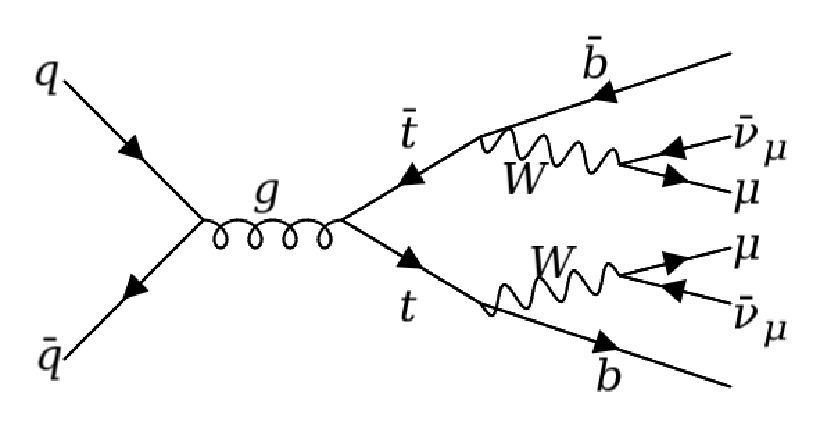
\includegraphics[width=\textwidth]{../figures/qqscattering.pdf}
		\caption{$qq$ scattering to $t$ quarks via a gluon, and decaying those quarks to leptons via $b$ quarks and $w$ bosons.}
		\label{fig:qqscattering}
	\end{subfigure}
	\caption{Possible hard scattering processes for \texttt{Event 11}}
	\label{fig:possibleProc11}
\end{figure}
\FloatBarrier

\subsubsection{Event 20:}

In this event \ref{fig:event20}, $\slashed{E}_T$ has a value around $60$ GeV which shows the presence of a neutrino in this event. Also, on the right top there is a muon observed because it was detected on the muon spectrometer, and it deposit less energy around $2.2$GeV. On the right top part of the display, there is a particle which createad a EM shower on the ECAL, but no signnificant energy deposited on the HCAL. This particle could be a photon, positron, or an electron. However, It is known that there is always at least two leptons in each event, it is highly possible that this particle is not a photon. Because, there is no other muon detection and any other energy deposition on the ECAL, no other lepton candidate left on the display except the one create an EM shower on the top left. To sum up, in this event one $e^-$ (or $e^+$), one muon and one neutrino is obtained. This process can be explained by the weak interaction processes. For instance, $b$ quark decay as in eqn.\ref{bdecay}.

\begin{equation}
	b \rightarrow Wc \rightarrow e\nu_e Ws \rightarrow e\nu_e \mu\nu_\mu s
	\label{bdecay}
\end{equation}

This process can be seen from the fig.\ref{fig:bdecay}.

\begin{figure}[h]
    \centering
	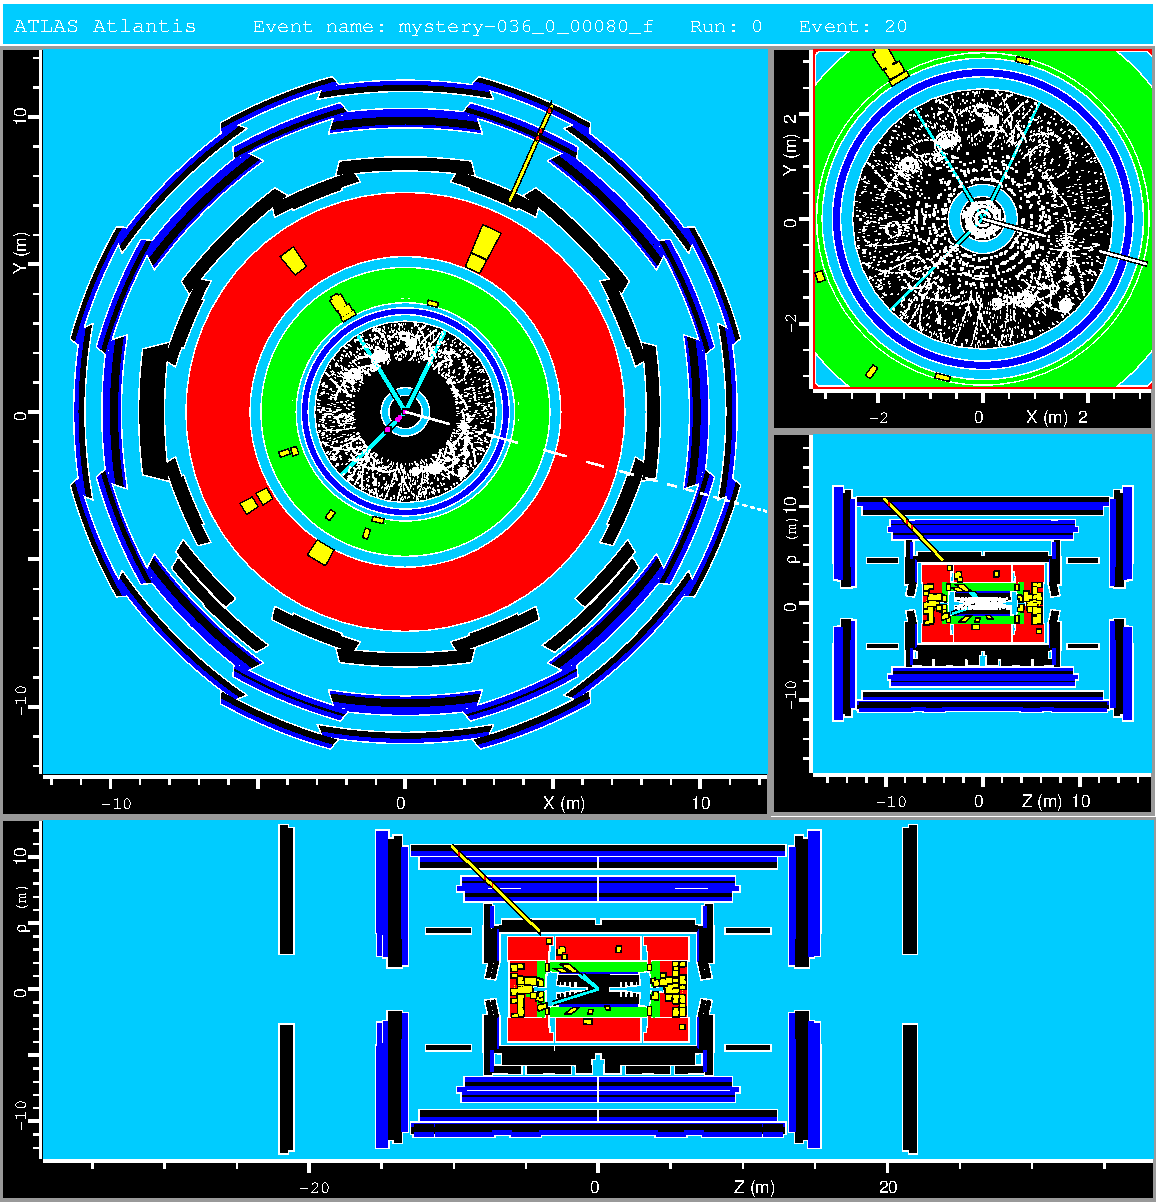
\includegraphics[width=0.5\textwidth]{../figures/mystery-event20.pdf}
	\caption{Mystery data set \texttt{Event 20}}
    \label{fig:event20}
\end{figure}
\FloatBarrier

\begin{figure}[h]
    \centering
	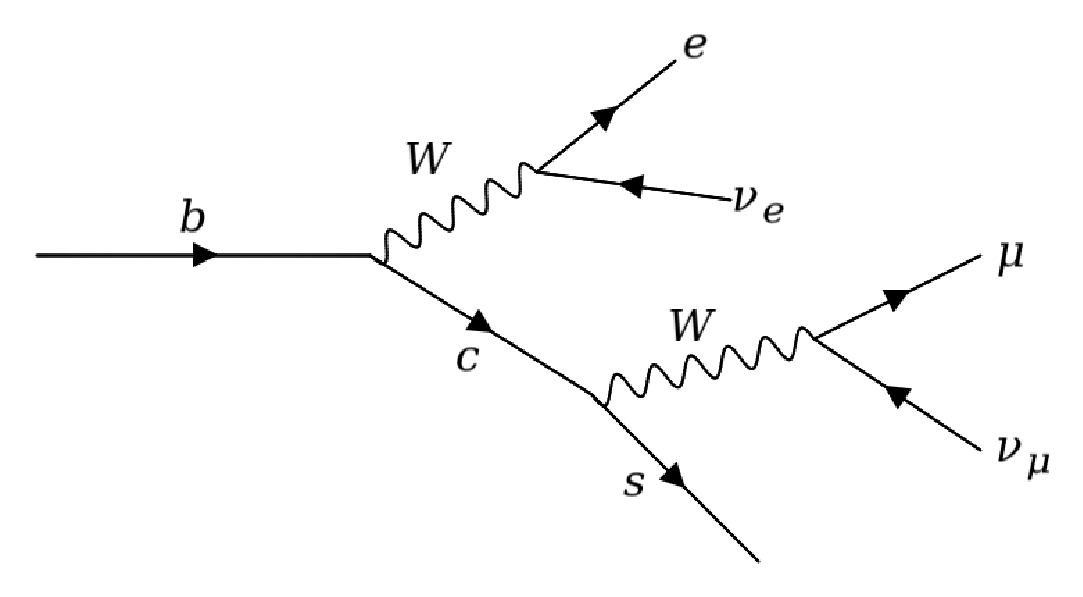
\includegraphics[width=0.5\textwidth]{../figures/bdecay.pdf}
	\caption{$b$ quark decay to weak interaction particle of $W$ bosons}
    \label{fig:bdecay}
\end{figure}
\FloatBarrier


\subsubsection{Event 45:}
In \texttt{Event 45} in the fig.\ref{fig:event45}, a high energy muon ($p_T$ equal to $81.3 \pm 7.8$ GeV) and a significant $ \slashed{E}_T $ of about $49$ GeV are observed, indicating the presence of a neutrino. In addition, there are two jet candidates in the event. Both of them deposited energy in both ECAL and only right bottom jet deposited energy on the HCAL, suggesting hadronic behavior. The jet bottom left appears to be an EM shower instead of a jet and it seems in the same track as the muon. These features point to a top quark decay scenario involving leptonic $W$ boson decay together with hadronic fragmentation originating from a $b$-quark ($t \rightarrow bW \rightarrow b\mu\nu$). Therefore, the claim that the event originated from a top-quark pair production process ($t\bar{t} \rightarrow b\mu\bar{\nu}\bar{b}+X$ as can be seen from fig.\ref{fig:qqscattering}) is strongly supported.

\begin{figure}[h]
    \centering
	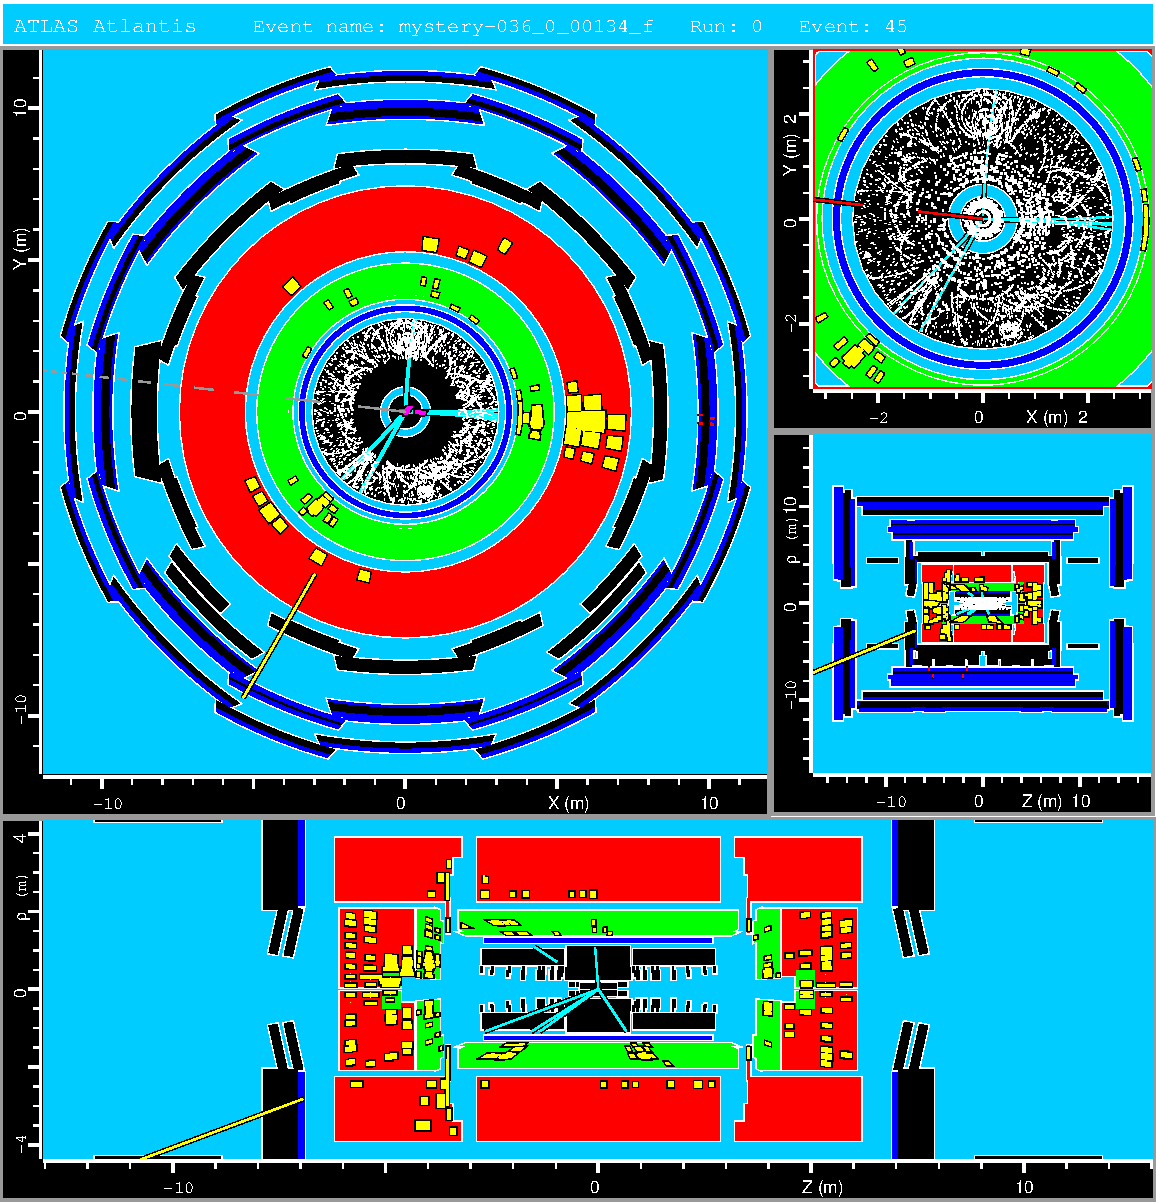
\includegraphics[width=0.5\textwidth]{../figures/mystery-event45.pdf}
	\caption{Mystery data set \texttt{Event 45}}
    \label{fig:event45}
\end{figure}
\FloatBarrier

\begin{table}[h]
		\centering
        \begin{tabular}{cc}
            \toprule
             product & Energy information [GeV]  \\
            \midrule
            bottom left $\mu$ & $p_T = 81.28 \pm 7.768$  \\
  			\midrule
  			bottom left jet & $ 52.4$(ECAL)  $ 3.0$(HCAL) \\
  			\midrule
  			bottom right jet & $ 65.3$(ECAL)  $ 24.0$(HCAL) \\
  			\midrule
			$\nu$ & $\slashed{E}_T = 48.891$ \\
			\bottomrule
        \end{tabular}
        \caption{Energy information of particles in \texttt{Event 11}, values were obtained via \texttt{ATLANTIS} program}
        \label{tab:event11}
    \end{table}
\FloatBarrier

\section{Calibration of Electrons}
Measuring the energy of electrons in an ECAL is the most sensitive way to determine their energy. However, the raw energy measurements given by the detector do not directly give accurate results and these data must be calibrated. The main reason for this is that the calorimeter consists of many parts and the energy responses of these parts may differ slightly from each other. In addition, electrons may lose energy in other areas of the detector before reaching the calorimeter, or some energy may be absorbed in the passive regions of the calorimeter. Due to these systematic effects, the ATLAS data sets provided in the laboratory contain only raw energy measurements, and these measurements are usually lower than the actual energy of the electron. Therefore, the electron energy must be calibrated. This calibration process will be carried out using the ROOT program in this laboratory study with the decay of $Z$ boson as $Z\rightarrow e^+e^-$ \cite{atlaslabmanual}. After this calibration done results are used to measure $W$ boson mass accurately. Because $W$ boson also decays leptons as $W\rightarrow e\nu$, which consists of electrons (or positrons).

\section{Calibration of Electron Energy}
\label{electroncalibration}
The electron energy calibration in the ATLAS calorimeter is done using the mass distribution of electron-positron pairs from the Z$^0$ boson. The properties of the Z$^0$ boson have been measured to high precision at the LEP collider, and its mass is known with a relative uncertainty of $\sim 2 \times 10^{-6}$ GeV. Therefore, the Z$^0$ peak of electron-positron events is a well-known signal and is used for calibrating the detector.

In an ideal detector, the invariant mass distribution $F(M_{ee})$ is modeled as:

\begin{equation}
	F(M_{ee}) = \frac{a}{M_{ee}^2} \left( \frac{1}{(M_{ee}^2 - M_Z^2)^2 + M_Z^2 \Gamma_Z^2} + F_{\text{Int}}(M_{ee}) + Bg(M_{ee}) \right)
	\label{eqn:invariantmass}
\end{equation}


Here $M_Z$ is the nominal mass of the Z$^0$ boson, $\Gamma_Z$ is the decay width. $F_{\text{Int}}(M_{ee})$ is the $\gamma$Z$^0$ interference term, and $Bg(M_{ee})$ is the background due to misidentified leptons\cite{atlaslabmanual}. Two approximation made, first one is $\gamma Z^0$ term is neglected, and second, standard Breit-Wigner, eqn.\ref{eqn:breitwigner} is used instead of relativistic one which is the $1^{st}$ term in the brackets in the eqn.\ref{eqn:invariantmass}

\begin{equation}
	F(M_{ee}) = \frac{\Gamma_Z^2 / 4}{(M_{ee} - M_Z)^2 + \Gamma_Z^2 / 4}
	\label{eqn:breitwigner}
\end{equation}

So, using the eqn.\ref{eqn:invariantmass} with eqn.\ref{eqn:breitwigner}, $\chi^2$ fit is applied and plot in fig.\ref{fig:eRawEnergyHist} was obtained.

The effect of this approach on the measurement is negligible. However, detector effects can systematically disturb the energy distribution by broadening this narrow peak. Depending on the region where the electron enters the calorimeter, the measured energy may deviate from the true energy \cite{atlaslabmanual}. The measured energy data can be seen from fig.\ref{fig:eRawEnergyHist}. Therefore, the calibration process is of great importance to correct the systematic errors of the detector.

\begin{figure}[h]
	\begin{subfigure}{0.5\textwidth}
		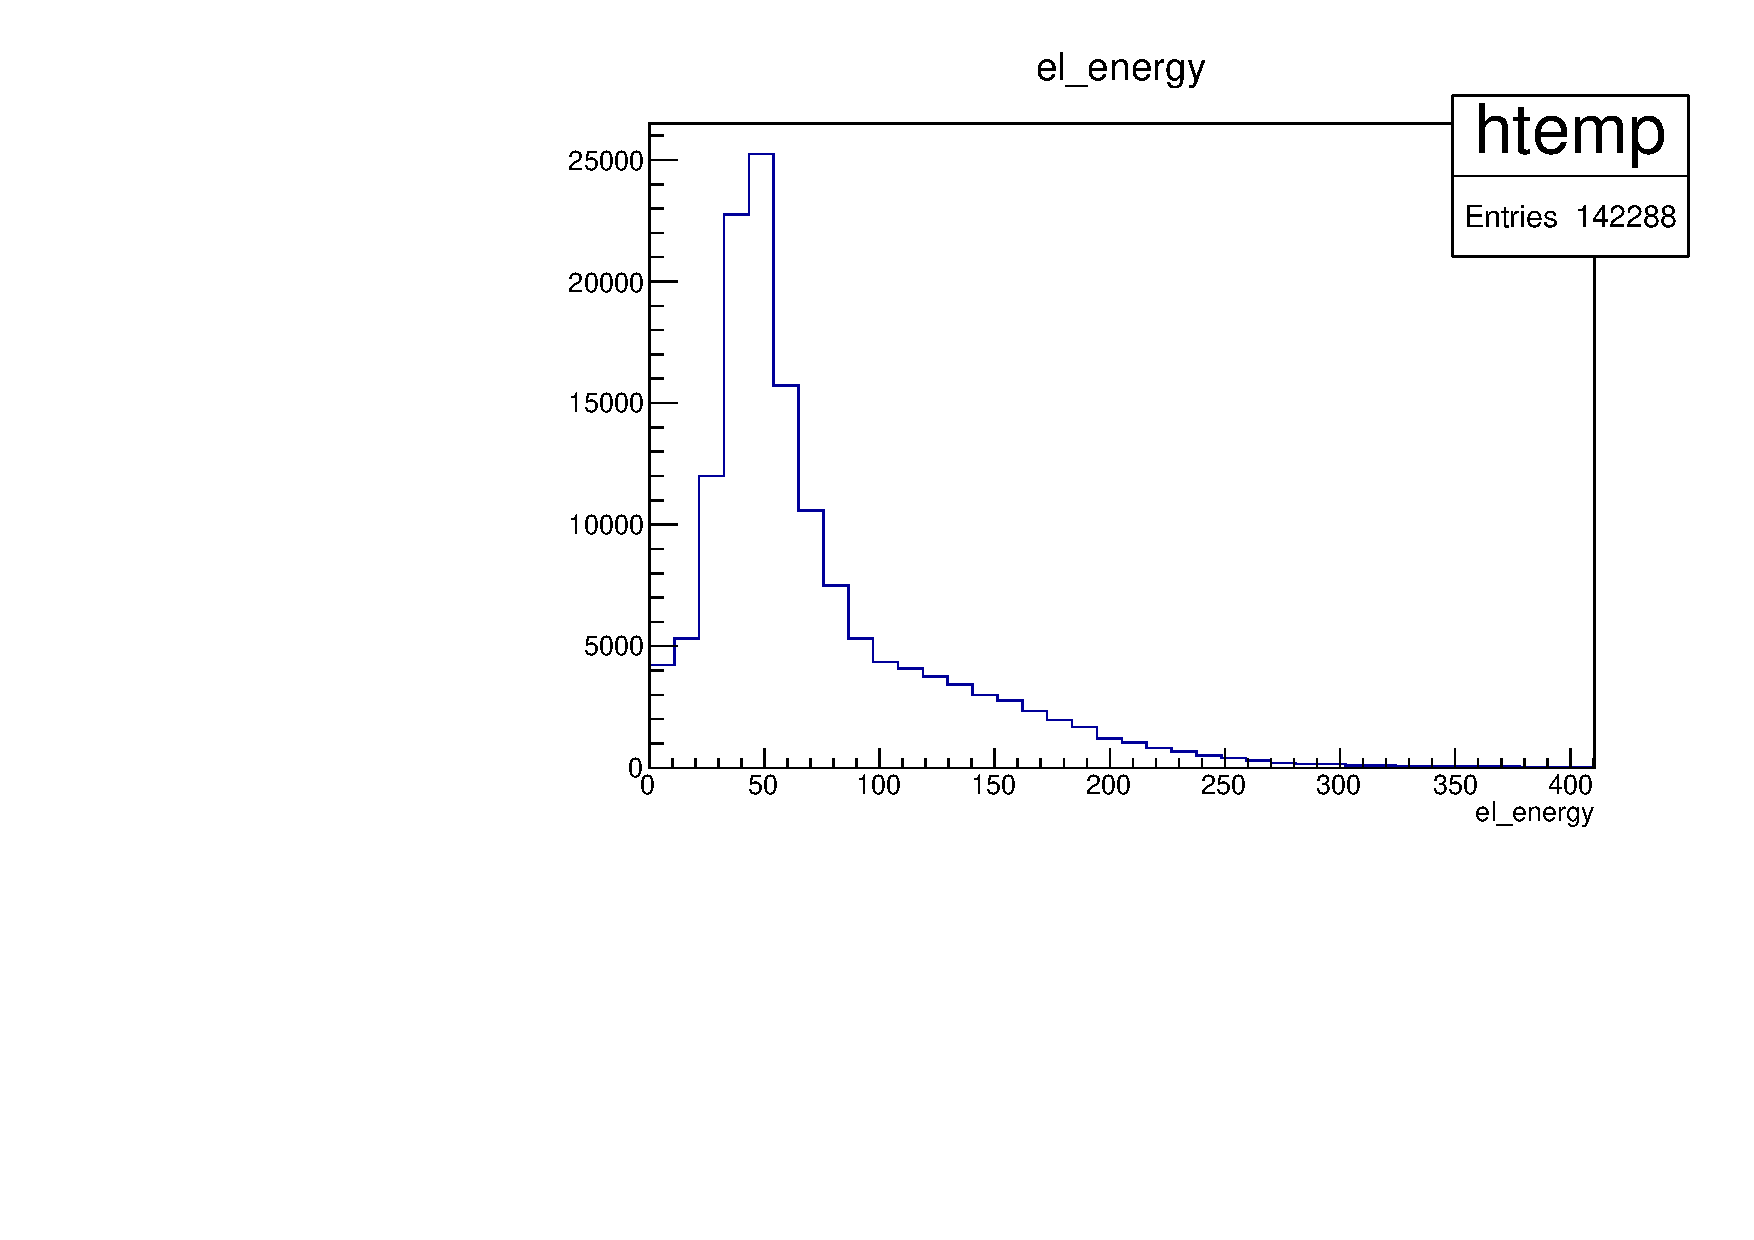
\includegraphics[width=\textwidth]{../figures/electron_E_histogram_raw.pdf}
		\caption{Raw Energy histogram of $e^-$}
    		\label{fig:e-rawEnergy}
	\end{subfigure}
	\hfill
	\begin{subfigure}{0.5\textwidth}
	 	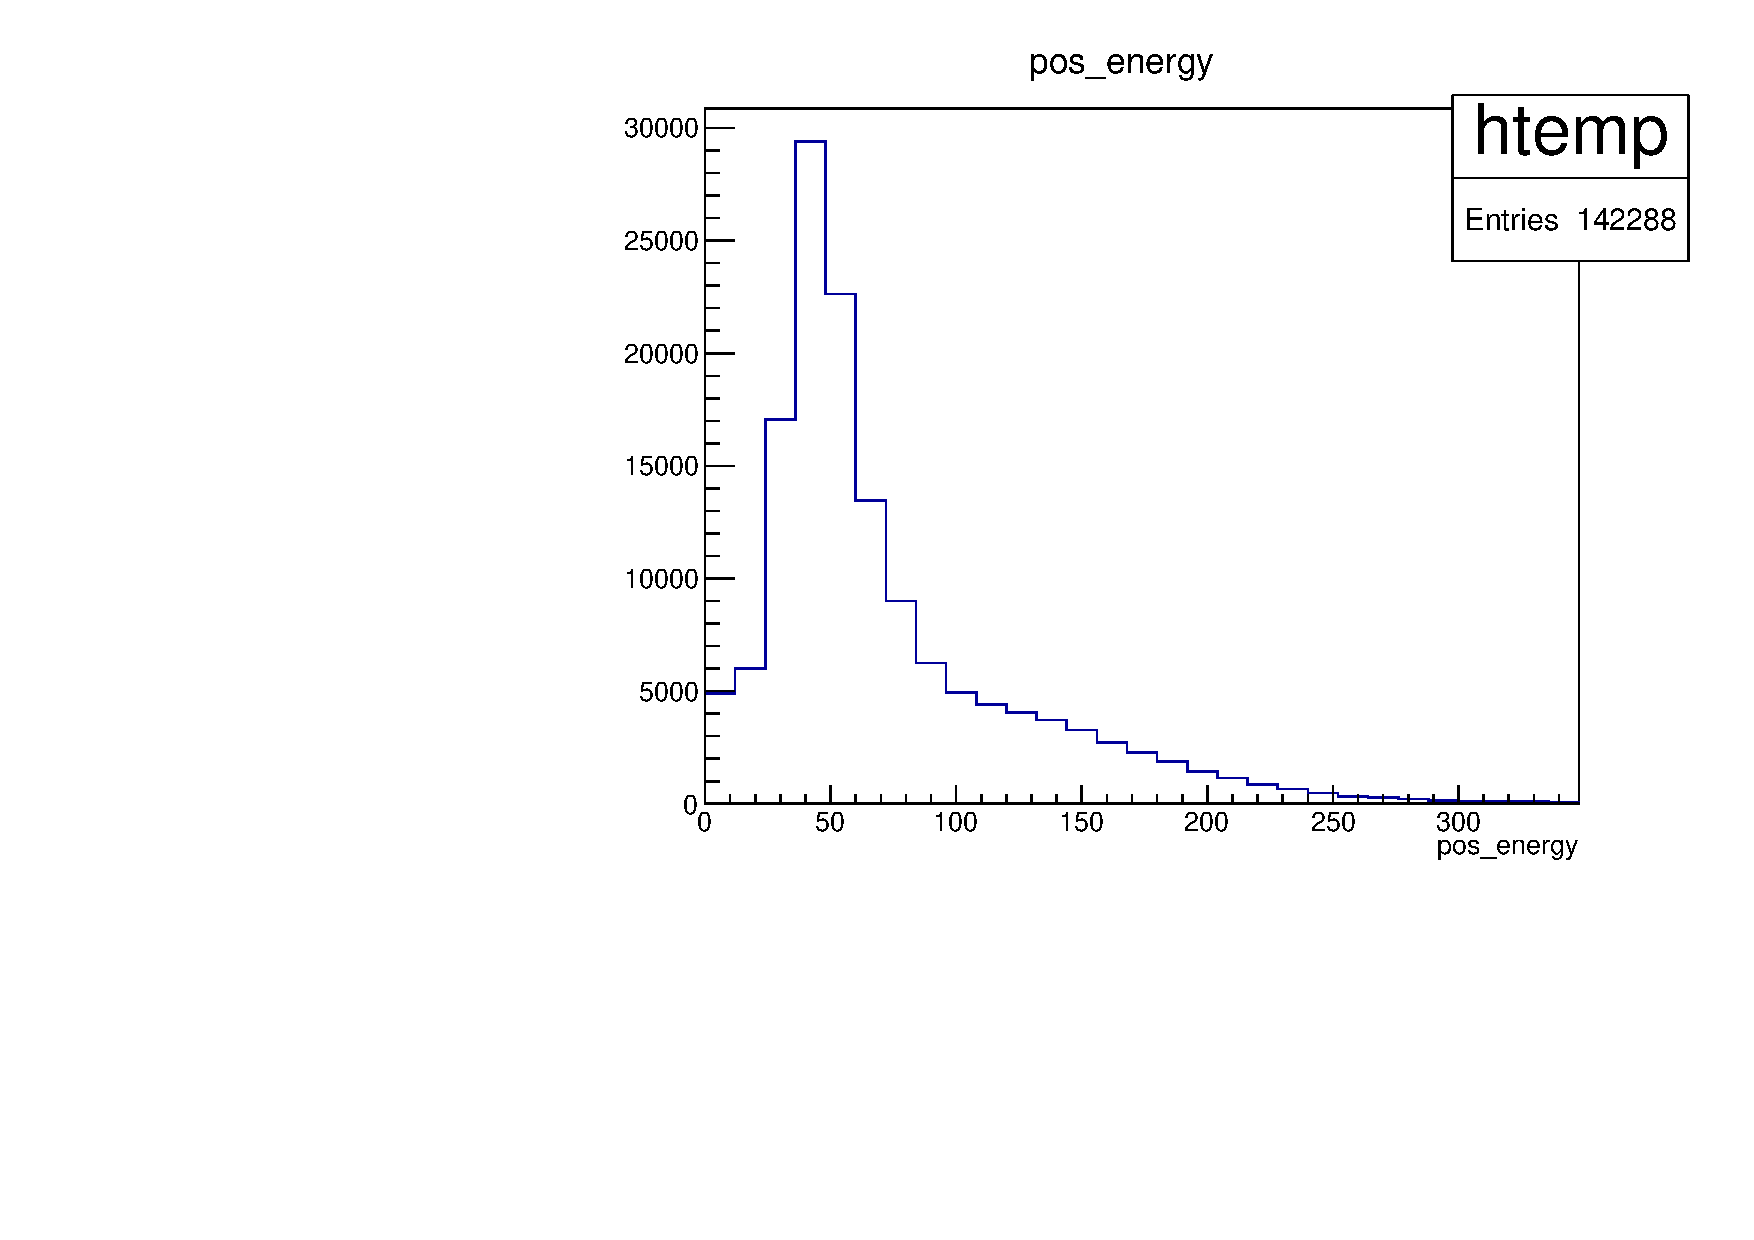
\includegraphics[width=\textwidth]{../figures/postitron_E_hist_raw.pdf}
		\caption{Raw Energy histogram of $e^+$}
		\label{fig:e+rawEnergy}
	\end{subfigure}
	\caption{Raw energy distributions of elektrons and positrons. Unit of horizantal axis is GeV and vertical axis is counts. As can be clearly seen that peak points of the both graphs are located around $50$GeV which is almost half of the mass of $Z$ boson}
	\label{fig:eRawEnergyHist}
\end{figure}
\FloatBarrier

Using the \texttt{ROOT} commands, necessary bins are applied to electron mass distribution. Positron mass distribution is similar to electron mass distribution, so seperate binnings were not applied to positron mass distribution. Without any binning selection, mass distribution of $Z$ boson can be seen from fig.\ref{fig:zfitraw}.

Here energy calibration done with a calibration factor defined as $\left(M_Z^{real} / M_Z^{meas}\right)$. When this calibration factor multiplied with raw energy, calibrated energy is obtained. $M_Z^{real}$ is the literature value which is taken to be reference to $Z^0$ boson mass. $M_Z^{meas}$ is measured $Z^0$ boson mass and it is obtained with different parameters as raw energy, transverse momentum ($p_T$), direction of electron $\phi$ and $\eta$, transversal energy in the calorimeter (\texttt{etiso}), ratio of electron-raw energy and electron momentum (\texttt{eoverp}), distance of the electron to the nearest jet in the $\eta\phi$ plane (\texttt{drjet}) \cite{atlaslabmanual}.
To do this calibration, first, energy plot with binning according to mentioned parameters done using \texttt{ROOT} commands. After looking this plot, measured energy value, $M_Z^{meas}$, is obtained and calibration parameter is calculated. For instance, $M_Z^{meas}$ value for $0.5<|\eta|<1.0$ is obtained from plot in the fig.\ref{fig:eta05-1bin} as $89.82 \pm 0.04$ GeV.

\begin{figure}[h]
    \centering
	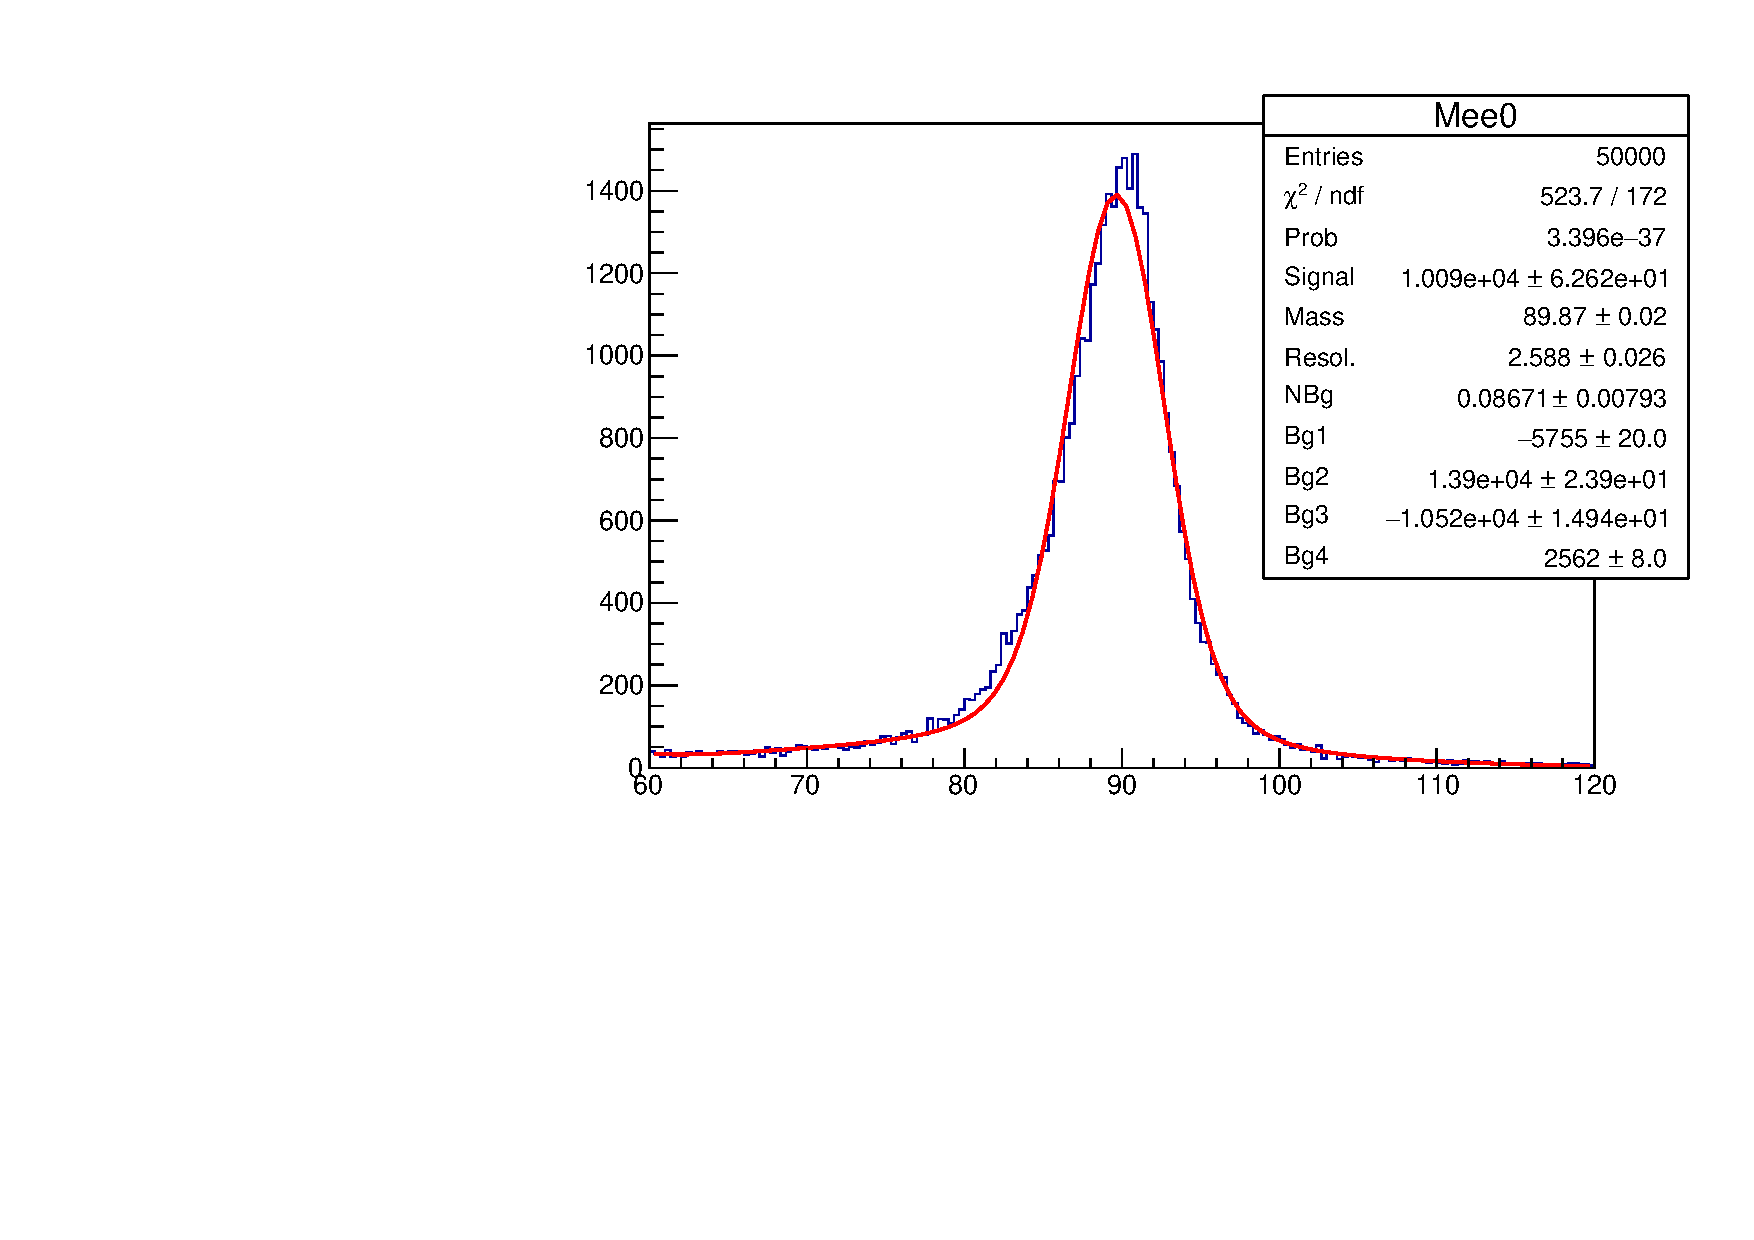
\includegraphics[width=0.8\textwidth]{../figures/z_fit_raw.pdf}
	\caption{Raw $Z$ mass distribution. Fit is applied according to convolution of a Gaussian function with a Breit-Wigner function which is eqn.\ref{eqn:breitwigner}. Unit of horizantal axis is GeV, vertical axis is counts.}
    \label{fig:zfitraw}
\end{figure}
\FloatBarrier

\begin{figure}[h]
    \centering
	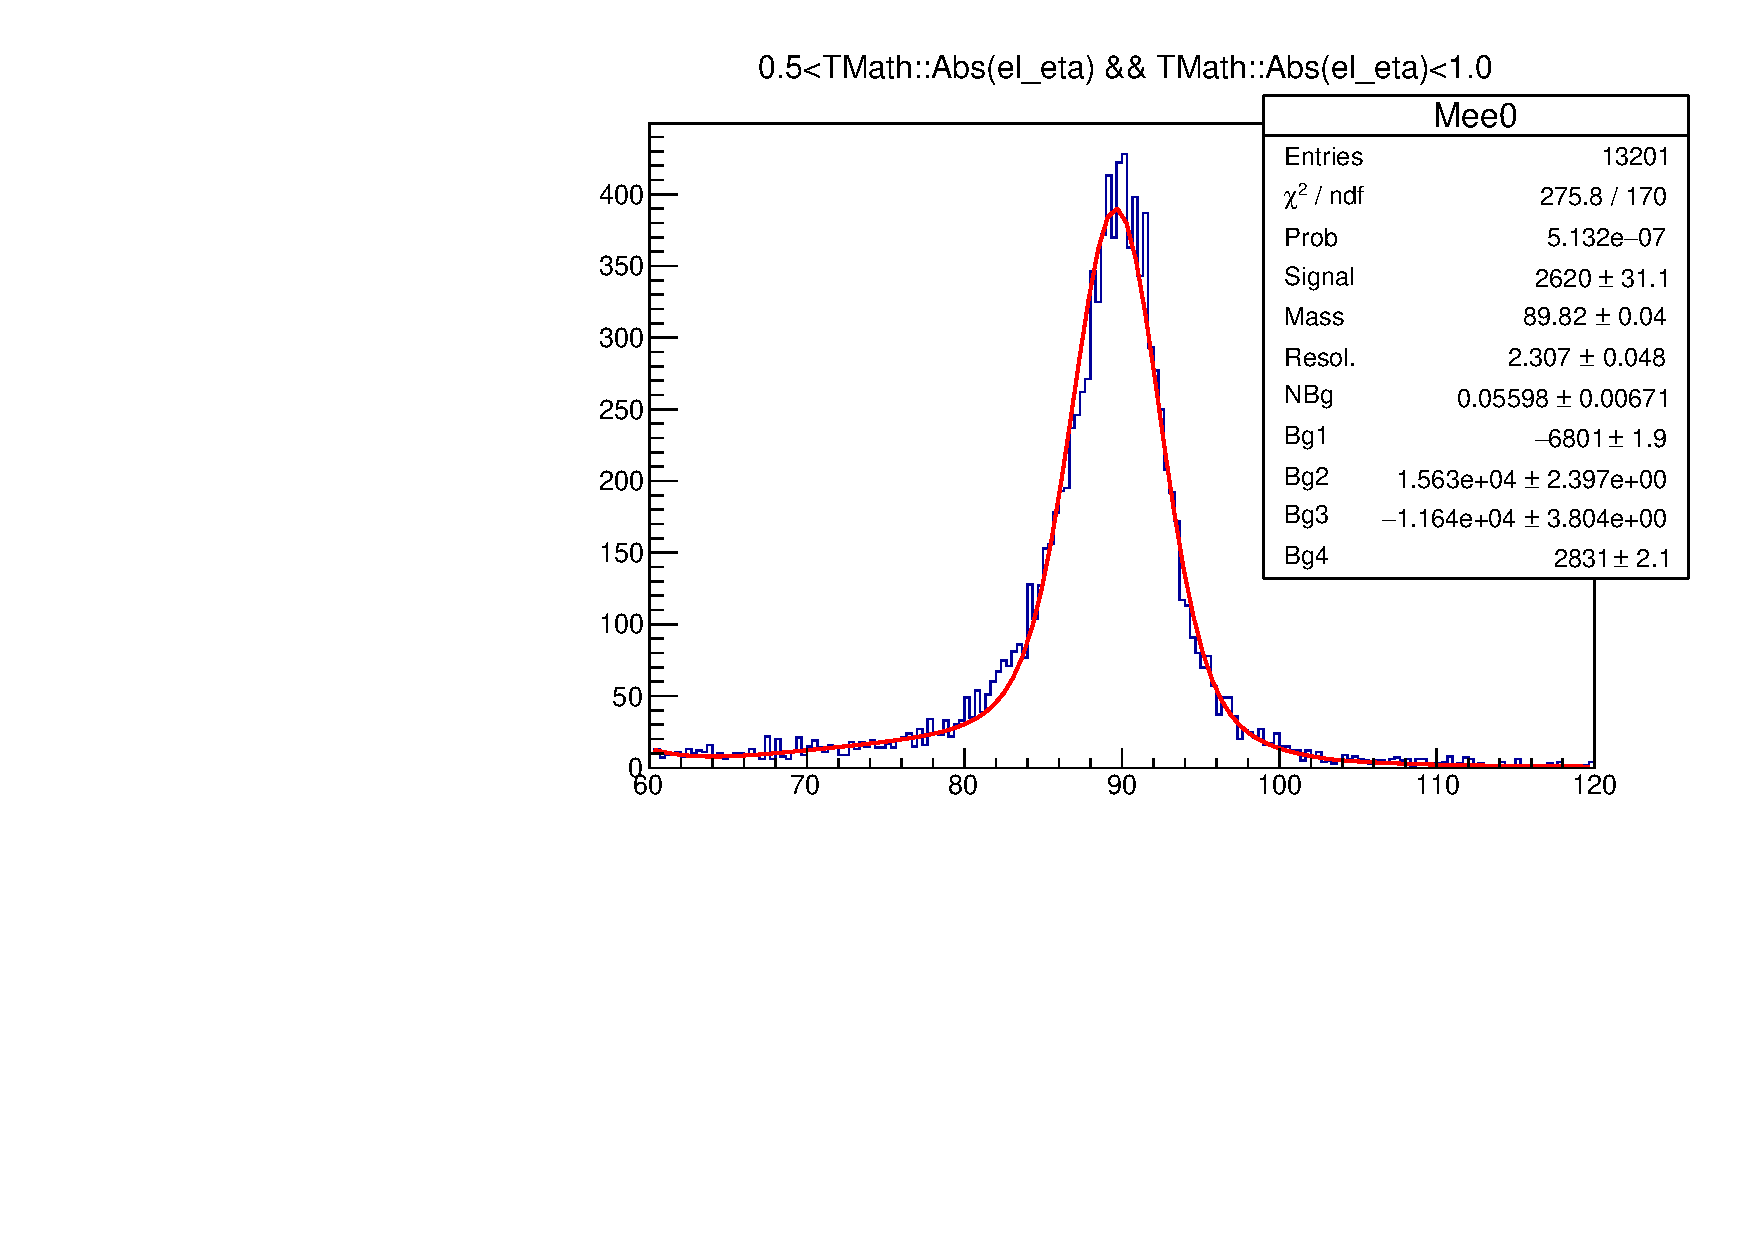
\includegraphics[width=0.8\textwidth]{../figures/eta_05-1_bin.pdf}
	\caption{$Z$ mass distribution with $0.5<|\eta|<1.0$. Unit of horizantal axis is GeV, vertical axis is counts.}
    \label{fig:eta05-1bin}
\end{figure}
\FloatBarrier

Initially, we have $ 89.87\pm0.02 $ GeV for $Z$ boson mass. This value has been tried to be improved for the exact value $M_{Z^0} = 91.1876 \pm 0.0021 \text{GeV/$c^2$}$\cite{pdg2018} with better $\chi^2 / ndf$ value which has to be approximately around $1$ for an ideal case. Following procedures were applied for improvement.

First, in the full $\eta$ range were bin with each $0.2$ increment which is considered as fine binning. Full code for this binning and the following ones can be seen in sec.\ref{sec:sectionB}.
\begin{figure}[h]
    \centering
	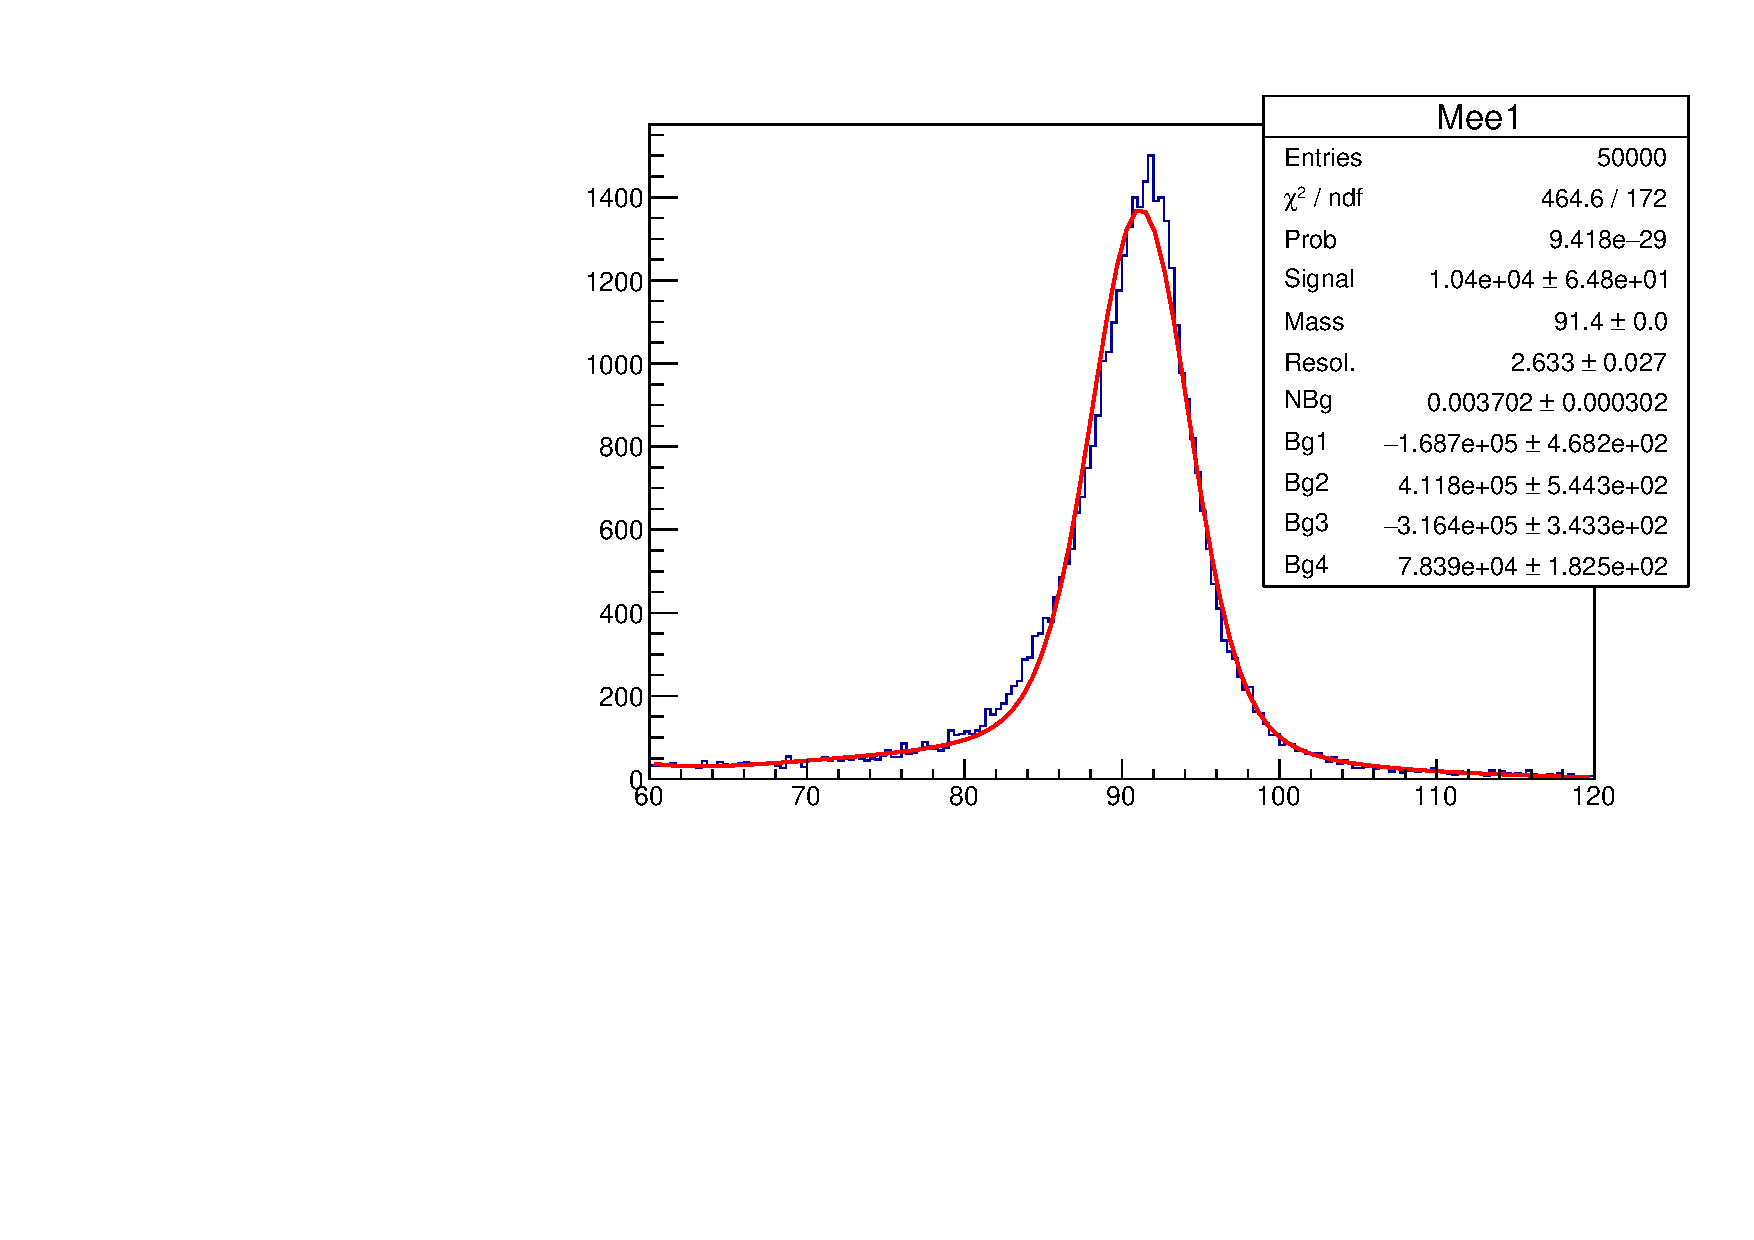
\includegraphics[width=0.8\textwidth]{../figures/full_eta_cuts.pdf}
	\caption{$Z$ mass distribution with fine binning of $\eta$. Unit of horizantal axis is GeV, vertical axis is counts.}
    \label{fig:full_eta_cuts}
\end{figure}
\FloatBarrier
As seen from the fig.\ref{fig:full_eta_cuts}, $Z$ boson mass calculated as $ 91.4 \pm 0.0 $GeV after fine cut. It was thought that energy value may be improved binning with two different parameters, and $\eta$ and raw energy values are used.
\begin{figure}[h]
    \centering
	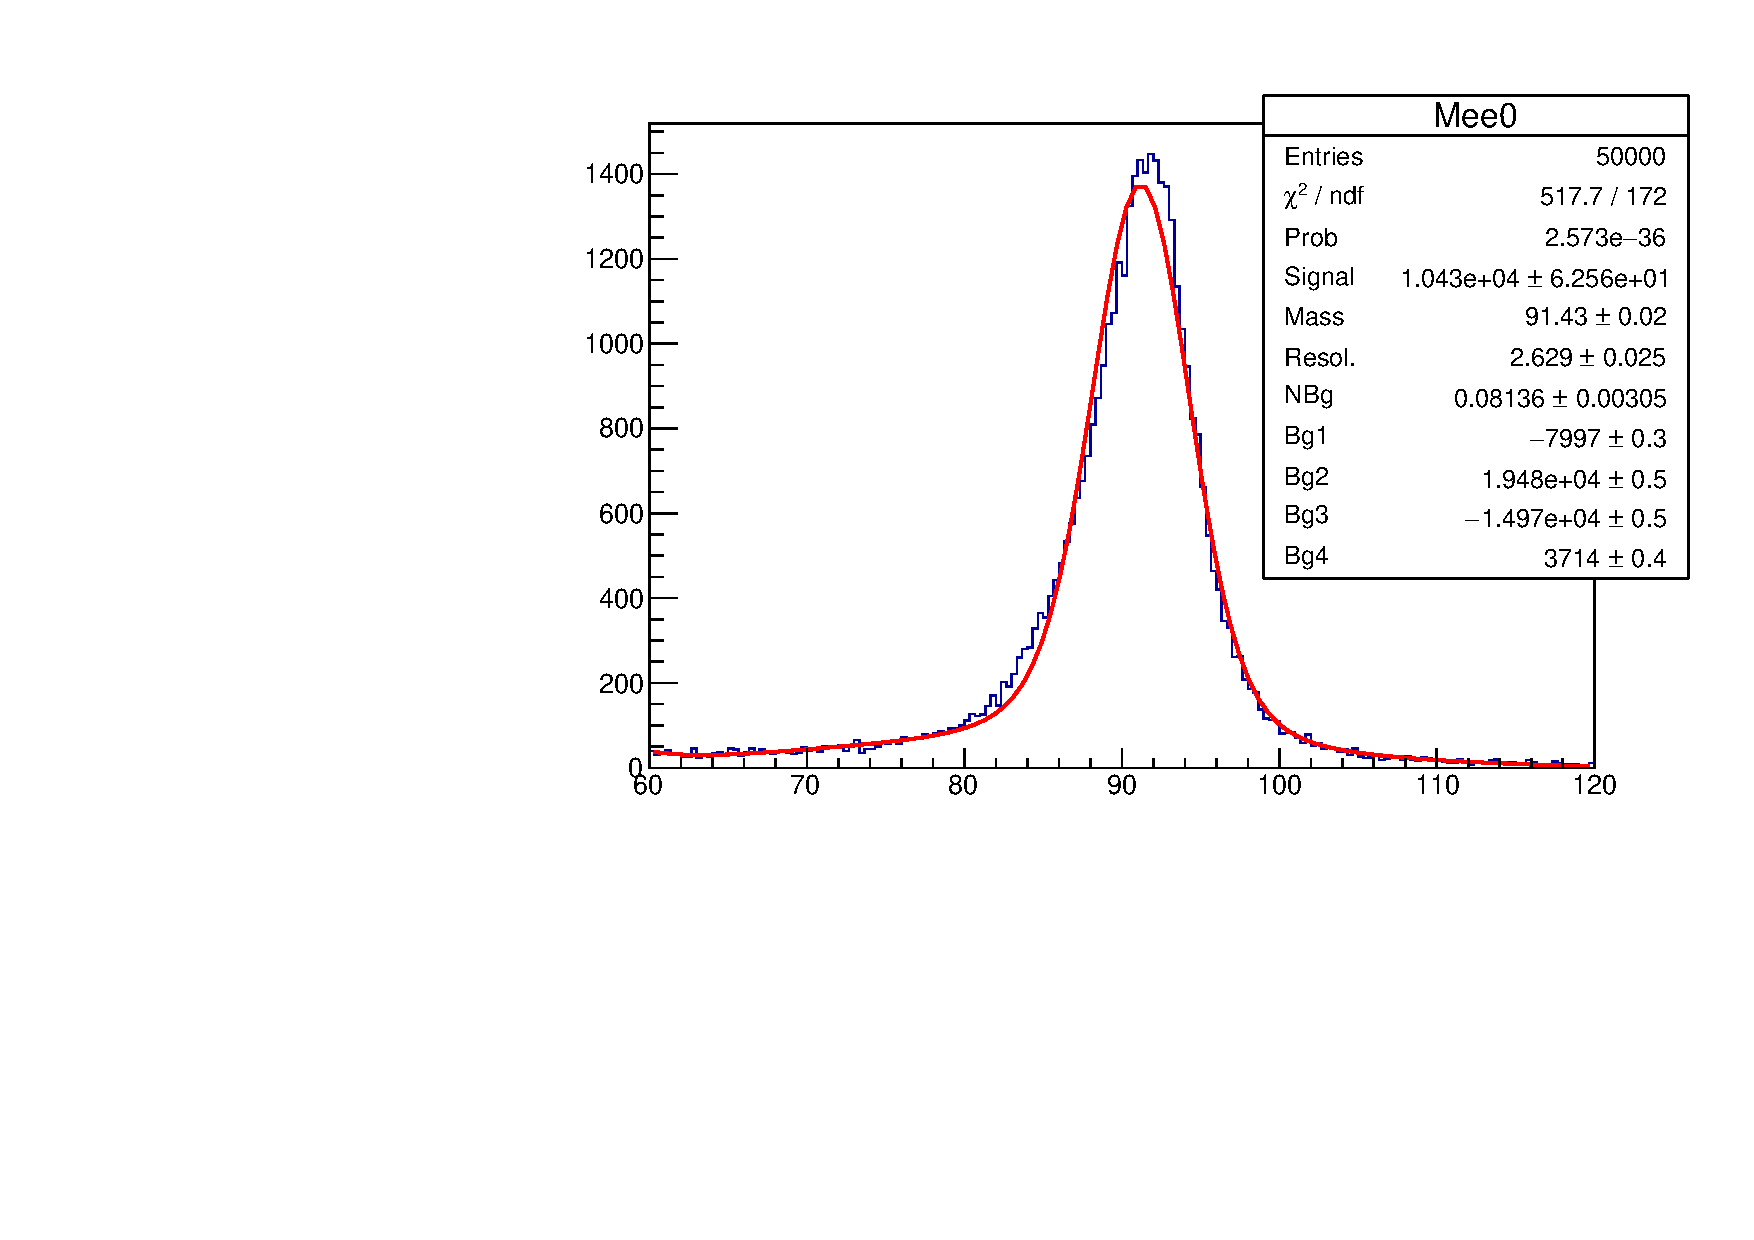
\includegraphics[width=0.8\textwidth]{../figures/energy_and_eta_cuts.pdf}
	\caption{$Z$ mass distribution with raw energy and $\eta$ binnings. Unit of horizantal axis is GeV, vertical axis is counts.}
    \label{fig:energy_and_eta_cuts}
\end{figure}
\FloatBarrier
For each $0.5$ increment of $\eta$, full energy range was binned from $30$ GeV to $70$ GeV with increment of $10$ GeV in a nested loop, and can be seen from sec.\ref{sec:sectionB}. After this binning, plot in fig.\ref{fig:energy_and_eta_cuts} was obtained. Here, in fig.\ref{fig:energy_and_eta_cuts}, $ 91.43 \pm 0.02$GeV. The obtained result getting worse with this approach so decided to stick one parameter, and after couple of trying on different parameters such as azimuthal angle $\phi$ and transverse momentum $p_T$, we decided to use $\eta$.
\begin{figure}[h]
    \centering
	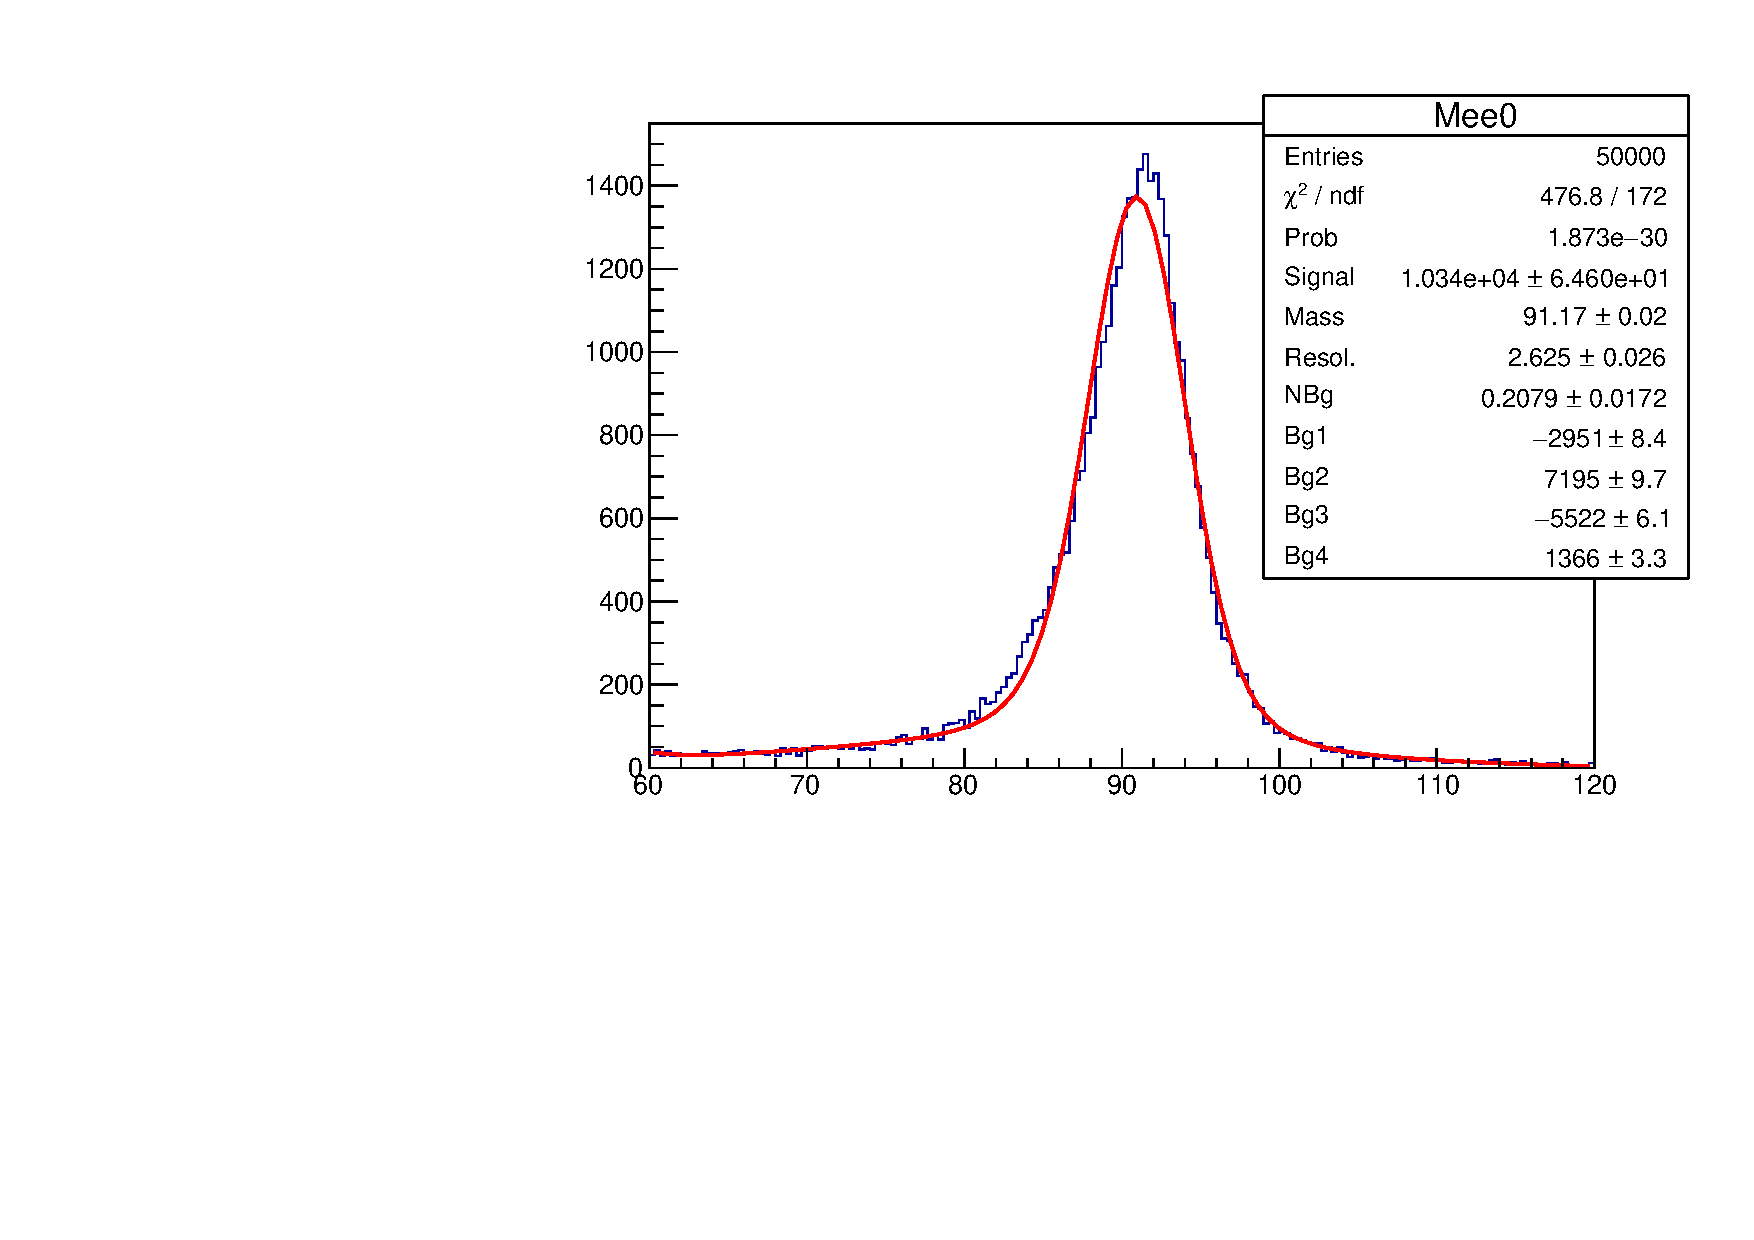
\includegraphics[width=0.8\textwidth]{../figures/course_eta_cuts.pdf}
	\caption{$Z$ mass distribution with coarse $\eta$ binnings. Unit of horizantal axis is GeV, vertical axis is counts. This distribution result used as calibration.}
    \label{fig:course_eta_cuts}
\end{figure}
\FloatBarrier
However, this time $\eta$ binned coarsely as $0.5$ increments as can be seen from the tab.\ref{tab:coarseETA}, also corresponding \texttt{C} code in \texttt{ElecCalib.c } can be seen from sec.\ref{sec:sectionB}
\begin{table}[h]
		\centering
        \begin{tabular}{ccc}
            \toprule
			Range &  Energy[Gev]   \\
            \midrule
            $ 0.0<|\eta|<0.5 $ & $ *= 91.2/90.18 $ \\
  			\midrule
  			$ 0.5<|\eta|<1.0 $ & $ *= 91.2/90.12 $ \\
  			\midrule
  			$ 1.0<|\eta|<1.5 $ & $ *= 91.2/89.80 $ \\
  			\midrule
  			$ 1.5<|\eta|<2.0 $ & $ *= 91.2/91.22 $  \\
  			\midrule
  			$ 2.0<|\eta|<2.5 $ & $ *= 91.2/88.72 $  \\
			\bottomrule
        \end{tabular}
        \caption{In each absolute value of $0.5$ $\eta$ range, energy value is updated with approximate exact value of $M_Z$ divided with each measured mass value $M_Z$ according to corresponding binning of $\eta$. }
        \label{tab:coarseETA}
    \end{table}
\FloatBarrier

Final calibrated mass of $M_Z$ is obtained as $91.17 \pm 0.02$ with $\chi^2 / ndf = 2.77$. Literature value of $M_{Z^0} = 91.1876 \pm 0.0021 \text{GeV/$c^2$}$\cite{pdg2018}. As expected, our error range is bigger than the literature value, however, $M_Z$ value we obtained stays inside the error range of  $M_Z$ value taken from literature. After this result, calibration accepted as done, and our result transfered to $W$ boson mass measurement part of the experiment by the tutor.

